%%
% 下のコメント欄は卒論執筆時の森がイキって書いたものです。
% 修論執筆時の森が代わりに謝罪いたします。
% 温かい目で見守ってあげてください。
%
% また、修論執筆時にはTeXstudioで、またDockerを用いて執筆しています。
% 上記の手法は平木場くんから教えていただきました。
% 参考: https://qiita.com/Shitimi_613/items/9706d57fb7bc17cbed0e
%

%%
% モダンなLaTeXを書きたい?
% そしたら僕の考えた最強のtexファイルを見てくれ
%
% 注意!
% このLaTeXをPDFに変換するためには、普通とはちょっと違う方法を使うよ
% コマンド上では
%   $ ptex2pdf -u -l GraduatePaper.tex
% で変換してね
% もしptex2pdfコマンドが無かったら、
%   $ uplatex GraduatePaper.tex
%   $ dvipdfmx GraduatePaper.dvi
% でうまくいくかも(未確認)
%
% え、TeXworksで使いたいって?
% そしたら、TeXworksの編集メニュー -> 設定を開く
% タイプセットタブの下の方にあるタイプセットの方法の右下の+ボタンを選択する
% 名前: uplatex(ptex2pdf)
% プログラム: ptex2pdf
% 引数: -l
%       -u
%       -ot
%       $synctexoption
%       $fullname
% として保存して、TeXworks実行ボタン右のコンボボックスのuplatex(ptex2pdf)を選択して変換だ!
%


%%
% 今時jarticleやjbook使ってる人いる?時代はjsarticleかjsbookだよ
% ついでに言うと、uplatexってのはplatexの上位互換、これを使わないなんて旧世代だよね
%
\documentclass[uplatex, report, a4j, 10pt]{jsbook}


%%
% パッケージ群
%
\usepackage{packages/miyazaki-u-paper}   % 宮崎大学工学部の卒論の基本(片山先生作)を、僕がちょっと書き換えちゃった(テヘッ
\usepackage{enumitem}           % enumerate?古い古い
\usepackage[dvipdfmx]{graphicx} % 当然dvipdfmなんて使ってないよね
\usepackage[dvipdfmx]{color}    % listingsを使うときにはこれも必須、dvipdfmxを変えちゃうとgraphicxのdvipdfmxも変わるよ
\usepackage{listings, packages/jlisting} % コードを埋め込むなら必須
\usepackage{txfonts}            % フォントといえばやっぱりtxfonts、今はnewtxってのもあるらしい
\usepackage{verbatim}           % コメントアウトしてくれる便利なプリアンブルが使える \begin{comment} ... \end{comment}
\usepackage[hdivide={21mm, , 21mm}, vdivide={30mm, , 25mm}]{geometry} % スタイルを少し変えたくても\hoffset, \voffsetは使わないでね
\usepackage[dvipdfmx]{hyperref}
\usepackage{pxjahyper}
\usepackage[htt]{hyphenat}

%\RequirePackage[l2tabu, orthodox]{nag} % これを入れると、古いコマンドを警告してくれる!なお完全には消せなかった模様
\newcommand\todo[1]{\PackageWarning{}{Detection TODO:#1}\textcolor{red}{(TODO:#1)}}

%%
% マクロの定義
%
\newcommand{\tool}{BWDM}
\newcommand{\toolFullName}{Verification tool for Vienna Development Method}

\renewcommand{\lstlistingname}{コード}
\lstset{
  language={Java},
  frame=tlBR,%フレーム線の指定、上右下左の順、大文字は二重線
%  frameround=tttt,%角の指定、右上|右下|左下|左上の順、tは丸角、fは四角
  framesep=5pt,%本文からframeまでの間隔
  framerule=.2pt,%線の太さ
%  rulecolor={\color[gray]},%線の色
%  backgroundcolor={\color[gray]{.9}},%背景色の指定
  basicstyle={\scriptsize\ttfamily \color[gray]{.15}},%書体の指定、この場合は7ptのタイプライタ体
  identifierstyle={\ttfamily},%識別子の書体
  keywordstyle={\ttfamily \color[cmyk]{0,1,0,0}},%言語ワードの書体
  stringstyle={\scriptsize\ttfamily \color[rgb]{0,0,1}},%文字列リテラルの書体
  commentstyle={\itshape \color[cmyk]{1,0,1,0}},%コメントの書体
  numberstyle={\scriptsize},%行番号の書式
  stepnumber=1,%行番号のステップ間隔
  numbers=left,%行番号の位置
  numbersep=1em,%本文との間隔
  breaklines=true,%改行の設定
  xleftmargin=0zw,
  xrightmargin=0zw,
  columns=[l]{fullflexible},
  lineskip=-0.5zw,
  morecomment={[s][{\color[cmyk]{1,0,0,0}}]{/**}{*/}},
  floatplacement=t,
  classoffset=1,
  showstringspaces=false,%空行の表示
%  breakatwhitespace=true,
%  tabsize=5,
}

\lstdefinestyle{interfaces}{
  float=tp,
  floatplacement=tbp,
  abovecaptionskip=-5pt
}

%%
% miyazaki-u-paper.sty用設定値
%
\degree{m} % Graduateのg or Masterのm
\figurenumbering{f} % 図目次を付ける場合はt (真) を持つ真偽値を引数に取る関数
\tablenumbering{f} % 表目次を付ける場合はt (真) を持つ真偽値を引数に取る関数
\title{VDM++仕様を対象としたテストケース \\ 自動生成ツールBWDMにおける \\ ペアワイズ法とドメイン分析テストの \\ 適用のための機能拡張}
\author{平木場 風太}
\nendo{1} % 年度
\advisor{片山 徹郎 教授} % 修論では無視する
\major{工学専攻 機械・情報系コース 情報システム工学分野}



\begin{document}
\maketitle

\preface{概要}

\todo{ここには概要を書く}


%%
% 本文
%
% はじめに
\chapter{はじめに}\label{cha:Introduction}
\todo{はじめにを書く}

以下、本論文の構成は次のとおりである。

第\ref{cha:Preparation}章では、\tool{}を実装するために必要となる前提知識について説明する。

第\ref{cha:Exist}章では、既存の\tool{}について説明する。

第\ref{cha:Extended}章では、拡張した\tool{}について説明する。

第\ref{cha:Indication}章では、拡張した\tool{}が正しく動作することを検証する。

第\ref{cha:Evaluation}章では、拡張した\tool{}について考察する。

第\ref{cha:Conclusion}章では、本研究のまとめと今後の課題を示す。



% 研究の準備
\chapter{研究の準備}\label{cha:Preparation}

本章では、\tool{}を実装するにあたり、必要となる前提知識を説明する。

\section{VDMJ}\label{cha:vdmj}
\todo{VDMJに関することを書く。既存のBWDM、拡張したBWDMの章で説明したこともこっちで書くべきかもしれない。}

\subsection{VDMJのクラス}\label{sec:vdmj_class}
\begin{table}[t]
  \begin{center}
    \caption{VDM++における定義、および、定義に対応するVDMJでの呼び方}
    \label{tab:vdmj_definition_name}
    \begin{tabular}{c|c}
      VDM++における定義    & VDMJでの呼び方     \\
      \hline
      \hline
      関数定義             & explicit function  \\ \hline
      操作定義             & explicit operation \\ \hline
      定数定義             & value              \\ \hline
      インスタンス変数定義 & instance variable
    \end{tabular}
  \end{center}
\end{table}

本研究で利用するVDMJのクラスを以下に示す。

\begin{itemize}
  \item 抽象クラス\texttt{VDMJ::TCDefinition}\\
        VDM++における各定義ブロックを表す抽象クラスである。フィールド\texttt{name}の値は定義名を示す。メソッド\texttt{kind()}を実行することで、定義の種類を取得できる。
        定義の種類を\ref{tab:vdmj_definition_name}に示す。
  \item クラス\texttt{VDMJ::TCExplicitFunctionDefinition}\\
        VDM++における関数定義ブロックfunctions内にある定義を表すクラスである。
  \item クラス\texttt{VDMJ::TCExplicitOperationDefinition}\\
        VDM++における操作定義ブロックoperationsにある定義を表すクラスである。
  \item クラス\texttt{VDMJ::TCValueDefinition}\\
        VDM++における定数定義ブロックvaluesにある定義を表すクラスである。
  \item クラス\texttt{VDMJ::TCInstanceVariableDefinition}\\
        VDM++におけるインスタンス変数定義ブロックinstance variablesにある定義を表すクラスである。
\end{itemize}


\section{因子と水準}\label{sec:factor_and_level}
\todo{因子と水準の説明を書く}

\section{ドメイン分析テスト}\label{cha:domain}
本研究における、ドメイン分析テストの定義と、ドメインテストが必要となる仕様の例を、以下で示す。

\subsection{定義}\label{sec:define}
本研究におけるドメイン分析テストとは、関係性がある複数の変数を同時にテストする方法である\cite{izon}\cite{jstqb}。
ドメインとは、入力するデータの定義域である。
ドメイン分析とは、入力する変数と条件式を分析し、ドメインを抽出することである。
ドメイン分析テストでは、ドメインごとにonポイント、offポイント、inポイント、outポイントと呼ばれる入力値、および、それを元にしたテストケースを作成し、テストする。
境界値とは、同値分割した領域の端、あるいは端のどちらか側で最小の増加的距離にある入力値、または、出力値である\cite{jstqb}。
本研究では、境界値の中でも、条件式を満たす境界値を利用する。これを、TB(True Boundary)と命名する。
TBの定義を、以下に示す。
$condition$を条件式、$exp$を左辺、$int$を右辺とする。
\begin{itemize}
  \item $condition$が$exp = int$のとき、$TB = int$とする。
  \item $condition$が$exp < int$のとき、$TB = int - 1$とする。
  \item $condition$が$exp > int$のとき、$TB = int + 1$とする。
  \item $condition$が$exp <= int$のとき、$TB = int$とする。
  \item $condition$が$exp >= int$のとき、$TB = int$とする。
\end{itemize}
それぞれのポイントの定義を、以下に示す。
\begin{itemize}
  \item onポイント:着目条件式(後述)のTBである。ドメインを決定づける条件式に付き1つ生成する。他のonポイントと重複してはならない。$targetExp$を着目条件式とすると、onポイントは、$targetExp = True$かつ$exp = TB$となる値でなければならない。
  \item offポイント:着目するonポイントに隣接し、TBでない値である。onポイントに付き複数(着目条件式に含まれる変数 $*$ 2)個存在する。$targetVar$を着目変数(後述)とすると、offポイントは、$targetVar + 1$となる値、または、$targetVar - 1$となる値でなければならない。
  \item inポイント:ドメインを決定づけるすべての条件式を満たす値である。ドメインに付き1つ生成する。onポイントやoffポイントと重複してはならない。$onPoints$をonポイントの集合とし、$offPoints$をoffポイントの集合、$inPoint$をinポイントとすると、inポイントは、 $(condition1 \land condition2 \land ... \land conditionN) = True$ かつ $inPoint \notin (onPoints \cup offPoints)$となる値でなければならない。
  \item outポイント:着目条件式のみを満たさない値である。ドメインを決定づける条件式に付き1つ生成する。offポイントと重複してはならない。$outPoint$をoutポイントとすると、outポイントは、$ (\lnot targetExp \land condition1 \land condition2 \land ... \land conditionN) = True$かつ$outPoint \notin offPoints$となる値でなければならない。
\end{itemize}
また、それぞれのポイントは、以下のパラメータを持つ。
\begin{itemize}
  \item 正常系判定値
        \begin{itemize}
          \item “正常系”とは、ポイントの期待出力がドメインの期待出力と一致する状態のことを言う。
          \item “非正常系”とは、ポイントの期待出力がドメインの期待出力と一致しない状態のことを言う。
          \item "正常系判定値"とは、正常系であるかどうかを保持する値である。正常系か非正常系かの2つの状態を持つ。
        \end{itemize}
  \item 着目条件式\\
        onポイント、offポイント、outポイントのみが持つ。どの条件式に着目してポイントを生成したかの情報である。
  \item 着目変数\\
        offポイントのみが持つ。どの変数に着目して、onポイントに隣接するポイントを生成したかの情報である。
\end{itemize}

\subsection{例}
\lstset{language=}
\noindent\begin{minipage}{\textwidth}
  \begin{lstlisting}[caption=ドメインテストが必要となる仕様(遊園地チケット割引機能),label=fig:vdm_park]
class 遊園地チケット

functions

static public 割引判定 : int * int -$>$ seq of char
  割引判定(夫の年齢, 妻の年齢) ==
    if(夫の年齢 + 妻の年齢 $<=$ 50) then
      if(夫の年齢 $>=$ 18) then
        if(妻の年齢 $>=$ 16) then
          ``割引価格となる''
        else
          ``割引価格とならない(妻の年齢 $<$ 16)''
      else
        ``割引価格とならない(夫の年齢 $<$ 18)''
    else
      ``割引価格とならない(夫の年齢 + 妻の年齢 $>$ 50)'';

end 遊園地チケット
\end{lstlisting}
\end{minipage}

ドメイン分析テストが必要となる仕様の例として、遊園地チケット割引機能をテストすることを考える。遊園地チケット割引機能は、夫婦である夫と妻それぞれの年齢を入力とし、割引価格が適用されるかどうかを判定する関数であり、以下のルールを持つ。
\begin{enumerate}
  \renewcommand{\labelenumi}{\Alph{enumi})}
  \item\label{enu:yuenchi} 以下の条件をすべて満たすとき、遊園地チケットは割引価格となる。
        \begin{itemize}
          \item 夫の年齢と妻の年齢の合計が50歳以下である。
          \item 夫の年齢は18歳以上である。
          \item 妻の年齢は16歳以上である。
        \end{itemize}
  \item A) でない場合、遊園地チケットは割引価格とならない。
\end{enumerate}
この仕様をVDM++で記述した仕様を、コード\ref{fig:vdm_park}に示す。
7行目に、複数の変数を左辺に含む条件式があるため、既存のBWDMではテストケース生成ができない。
また、“割引価格となる”というドメインの各ポイントを生成した例を、図\ref{fig:domain_points}に示す。
ドメインを決定づける3つの条件式は、“夫の年齢 + 妻の年齢 $<=$ 50”、“夫の年齢 $>=$ 18”、“妻の年齢 $>=$ 16”である。
onポイントは、“On1”〜“On3”の3つであり、それぞれ、条件式の境界線上に存在する。
offポイントは、“Off11”〜“Off32”の8つである。“Off11”〜“Off14”は“夫の年齢 + 妻の年齢 $<=$ 50”という条件式に着目した“On1”に隣接するoffポイントであり、4つ存在する。これは、“夫の年齢”を正負の方向にそれぞれずらしたoffポイントが2つ存在し、同じように、“妻の年齢”を正負の方向にそれぞれずらしたoffポイントが2つ存在するためである。
しかし、“On2”のoffポイントは“Off21”、 “Off22”の2つのみである。これは、“夫の年齢”をずらしたoffポイントが“妻の年齢 $>=$ 16”となり、TBとなるからである。
inポイントは、“In”の1つであり、“割引価格となる”ドメインのすべての条件式を満たす値を持つ。
outポイントは、“Out1”〜“Out3”の3つであり、それぞれの’着目条件式のみを満たさない値を持つ。

\begin{figure}[tp]
  \centering
  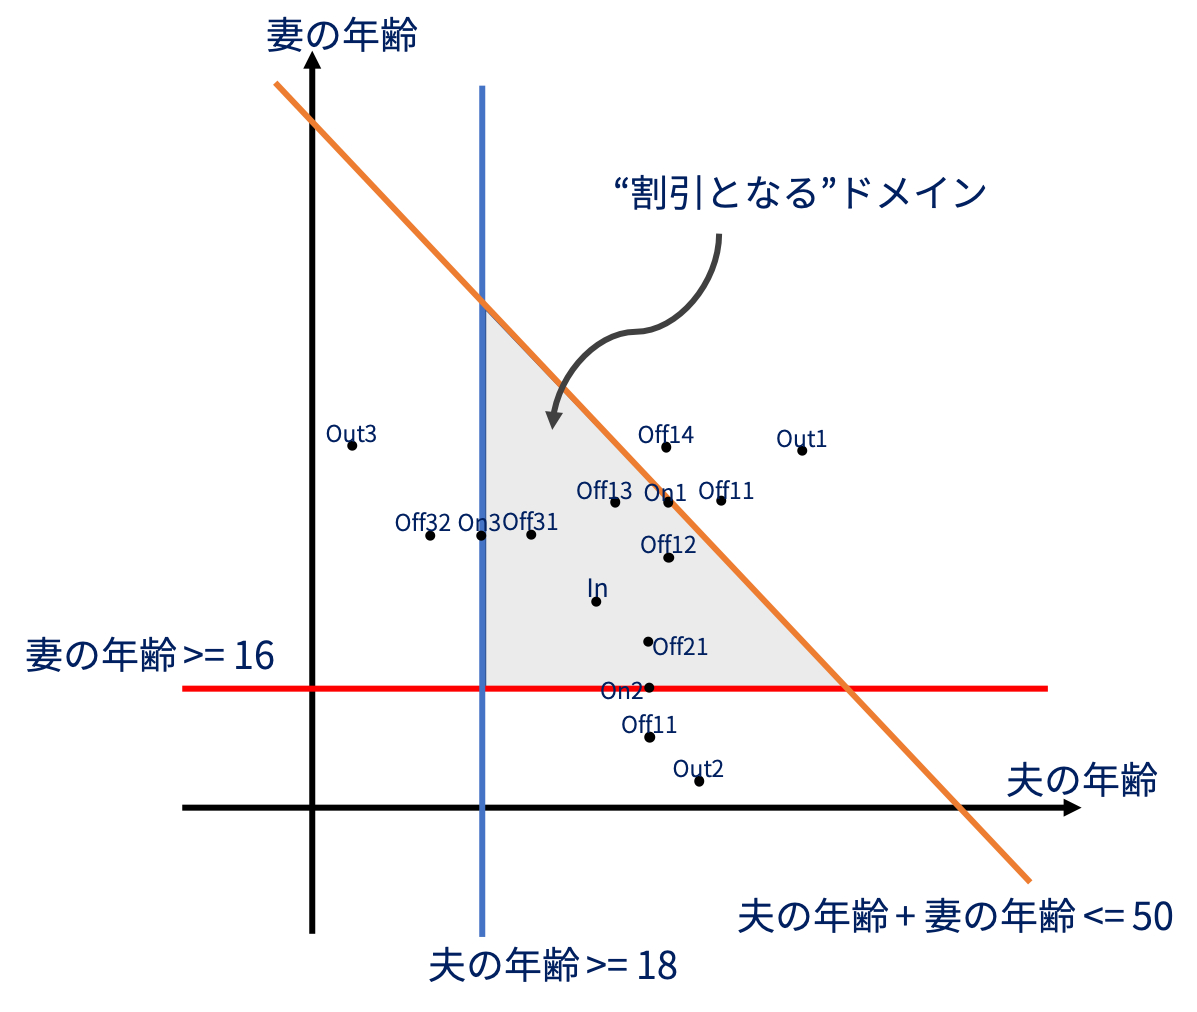
\includegraphics[keepaspectratio, width=160mm]{figs/domain_points}
  \caption{遊園地チケット割引機能( コード\ref{fig:vdm_park})の割引になる条件にドメイン分析を適用した例}
  \label{fig:domain_points}
\end{figure}



% 既存
\chapter{既存の\tool{}}\label{cha:Exist}
\todo{ぜんぜんBWDMの説明になっていないので、もっと既存のBWDMにできることを説明する。}

本章では、既存の\tool{} (\toolFullName{})について説明する。

\section{機能}
既存のBWDMには、以下の機能がある。

\begin{itemize}
  \item 記号実行によるテストケース生成
  \item 境界値分析によるテストケース生成
\end{itemize}

記号実行によって生成したテストケースは、すべての実行フローを網羅できることが期待できる。
境界値分析によって生成したテストケースは、境界値テストに使用することができる。
既存のBWDMを使用することにより、VDM++仕様を用いたソフトウェア開発効率を改善できる。

\begin{figure}[tp]
  \centering
  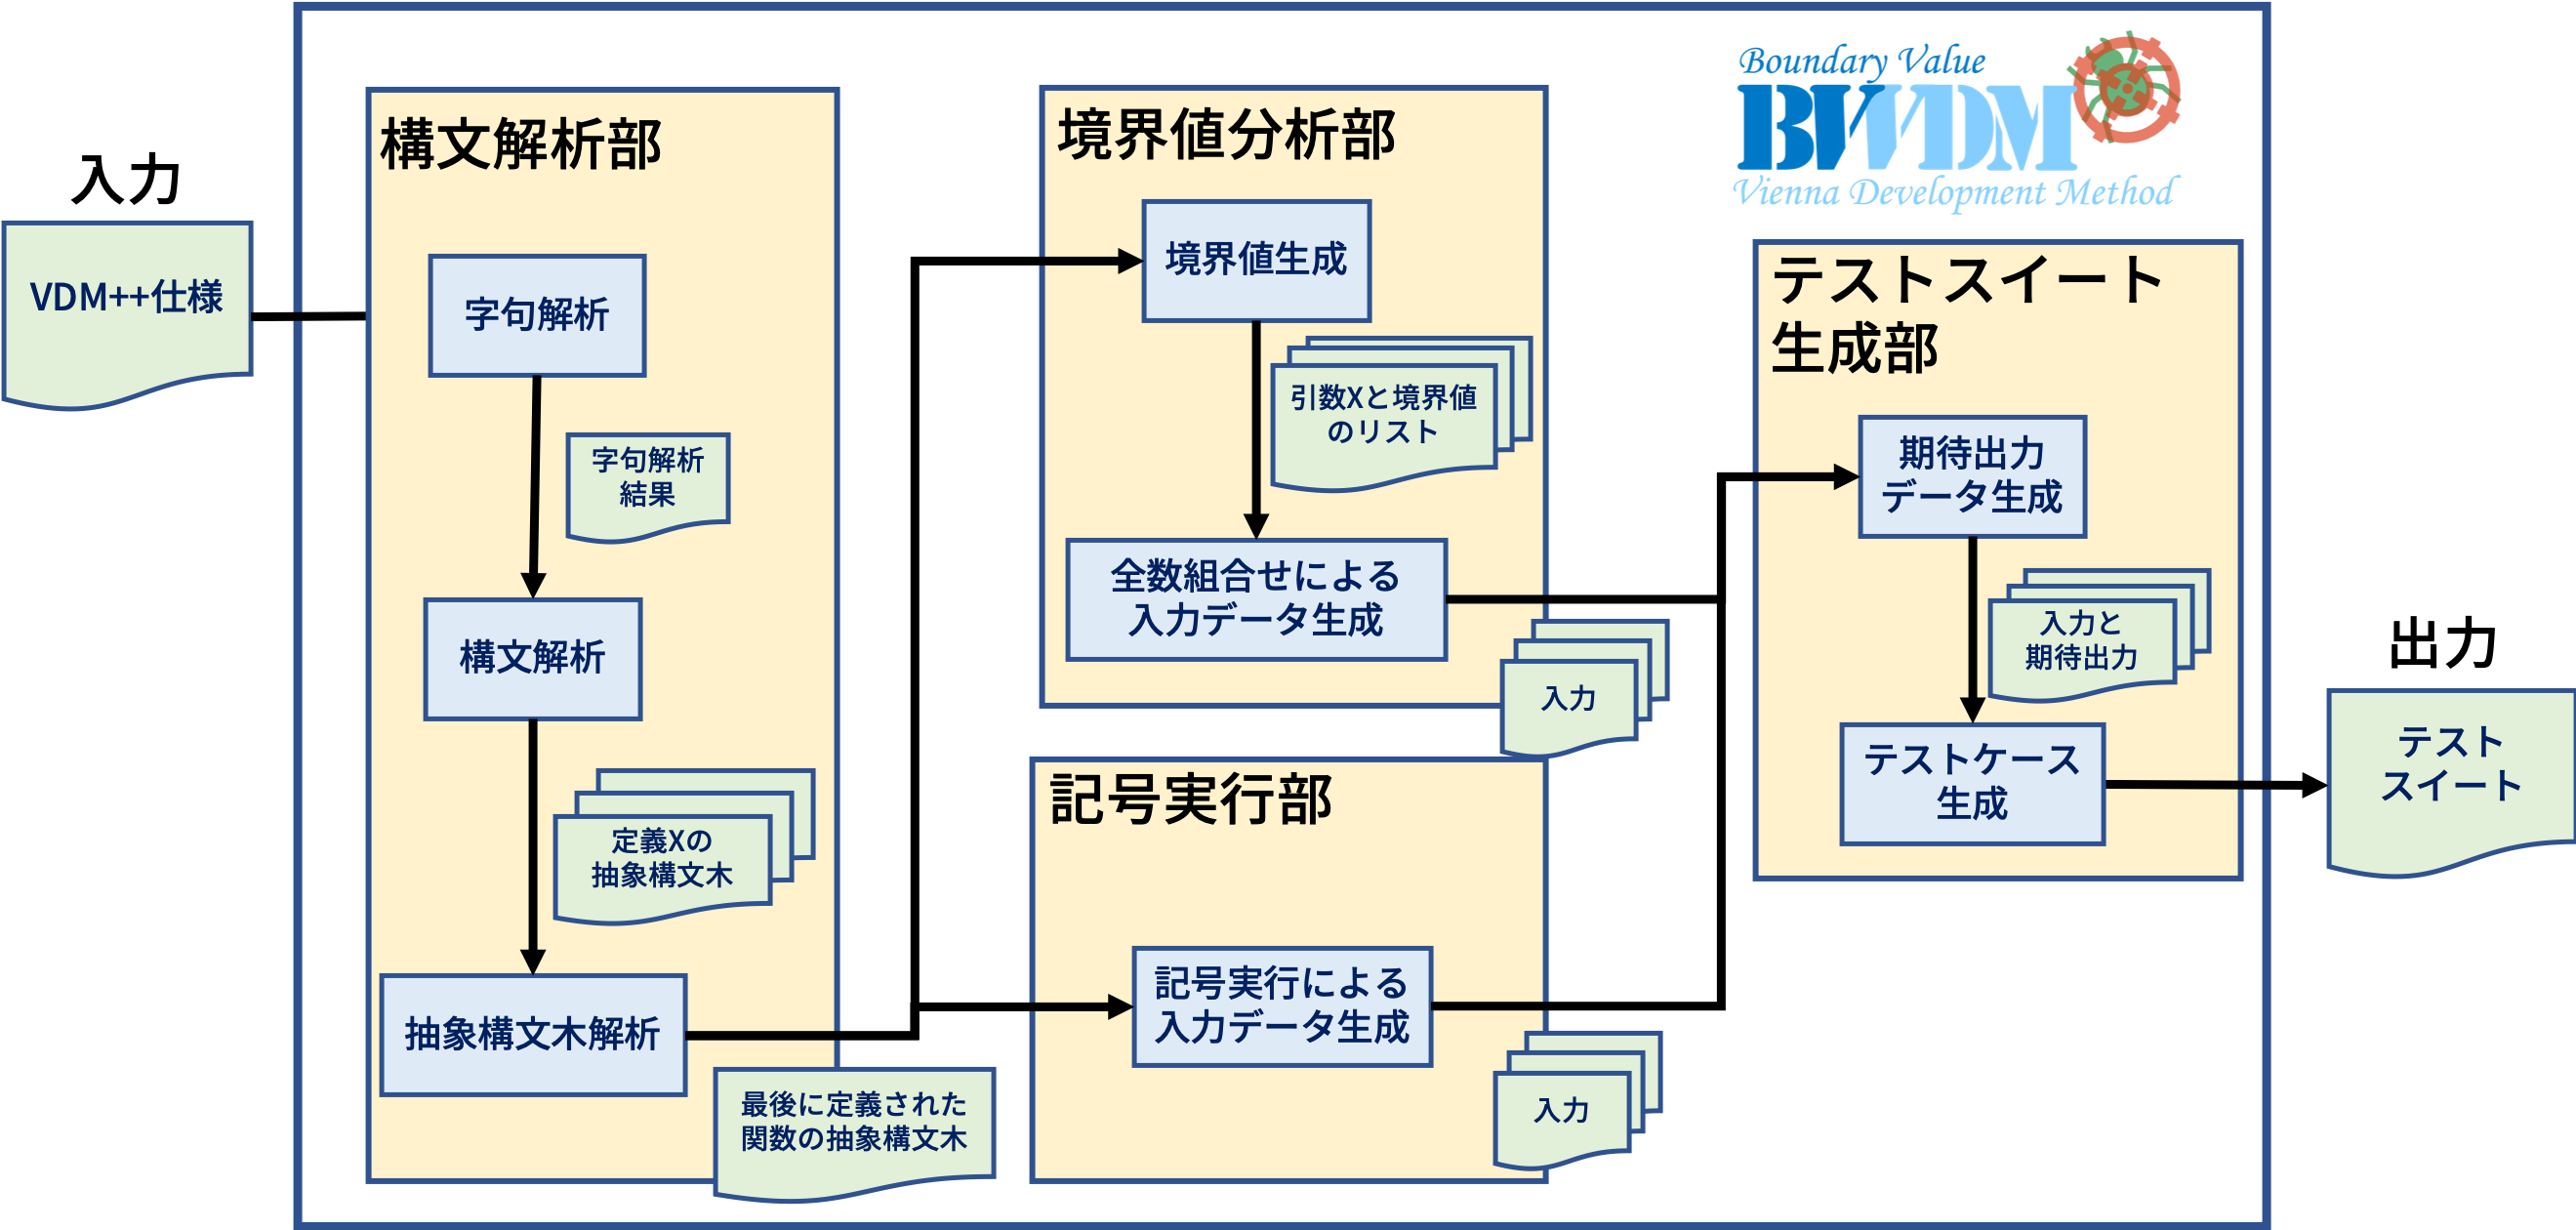
\includegraphics[keepaspectratio, width=160mm]{figs/exist_bwdm_structure.png}
  \caption{既存のBWDMの構造}
  \label{fig:existBwdmStructure}
\end{figure}

既存のBWDMの構造を図\ref{fig:existBwdmStructure}に示す。

\section{入出力例}

\lstset{language=}
\noindent\begin{minipage}{\textwidth}
  \begin{lstlisting}[caption=入力例:VDM++仕様,label=fig:input_sample]
class SampleClass

functions

sampleFunction : int*nat*nat $->$ seq of char
  sampleFunction(a, b, c) == 
    if(a $<$ 100) then
      if(b $>$ 2018) then
        "aは100未満かつbは2018より大きい"
      else
        "aは100未満かつbは2018以下"
    elseif(c $<$ 12) then
      "aは100以上かつcは12未満"
    else
      "aは100以上かつcは12以上";

end SampleClass

\end{lstlisting}
\end{minipage}

\begin{figure}[t]
  \begin{center}
    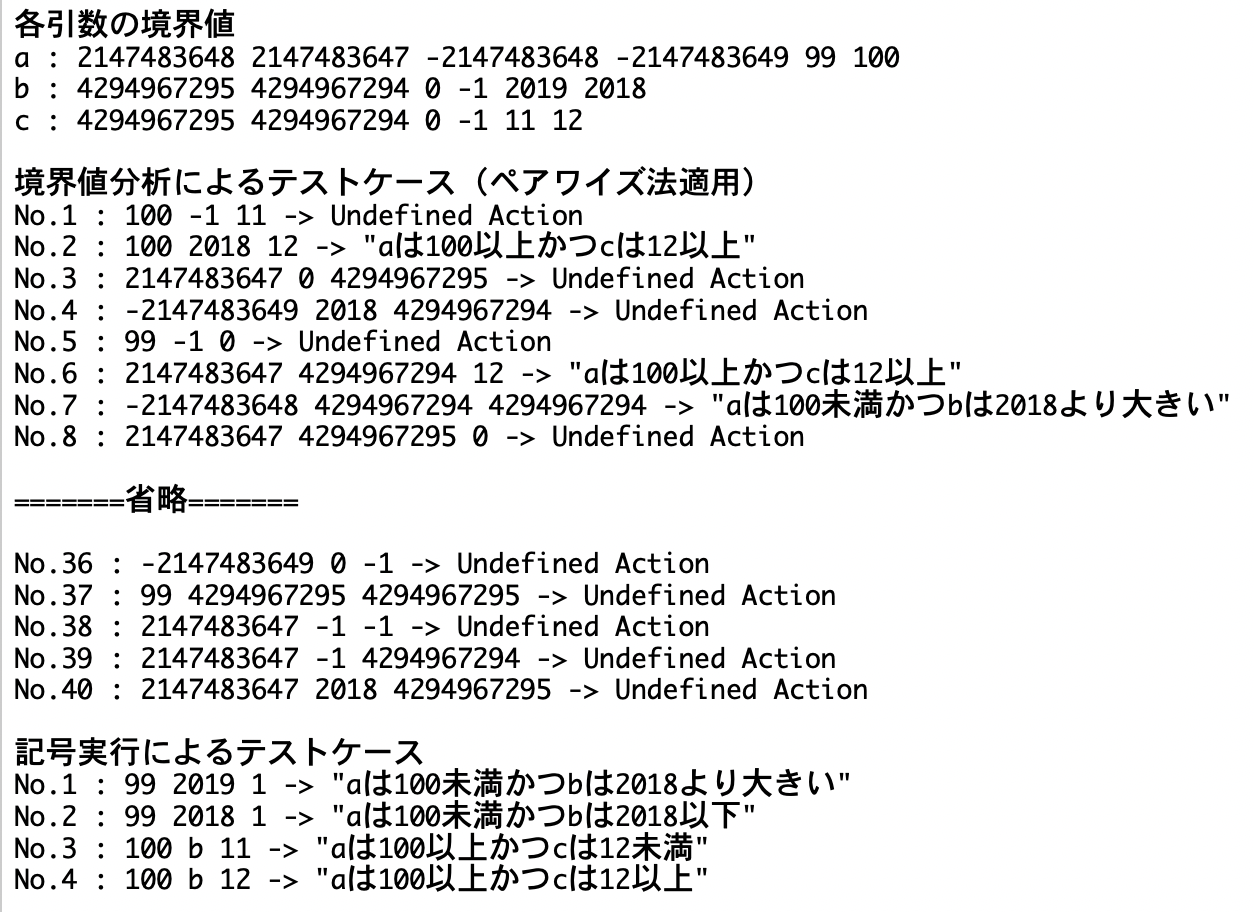
\includegraphics[keepaspectratio, width=160mm]{figs/sample_testcase.png}
    \caption{出力例:テストケース}
    \label{fig:testcase_sample}
  \end{center}
\end{figure}

\begin{figure}[t]
  \begin{center}
    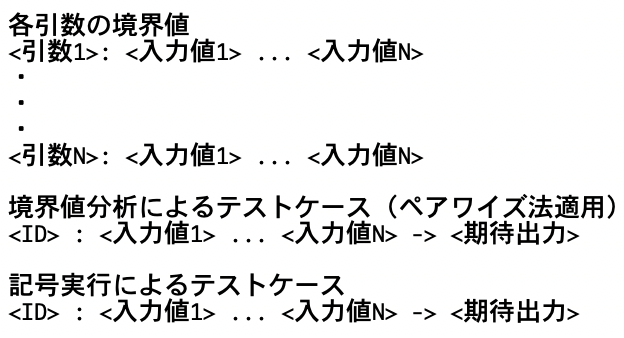
\includegraphics[keepaspectratio, width=160mm]{figs/bwdm_format.png}
    \caption{既存のBWDMのテストケースの出力フォーマット}
    \label{fig:bwdm_format}
  \end{center}
\end{figure}

VDM++仕様ファイルの例をコード\ref{fig:input_sample}に,
そのファイルから生成したテストケースの例を図\ref{fig:testcase_sample}に,それぞれ示す.
また,出力テストケースのフォーマットを,図\ref{fig:bwdm_format}に示す.
“各引数の境界値”にて,引数a, b, cそれぞれの境界値の集合を出力している.
そして,“境界値分析によるテストケース”にて,ペアワイズ法を用いて,各引数の境界値の組合せ総数を削減したテストスイートを出力している.
また,”記号実行によるテストケース”にて,関数のすべての実行フローを網羅できるテストスイートを出力している.

\section{問題}\label{sec:bwdm_problem}
既存のBWDMには問題がある。問題点を以下で説明する。

\subsection{組合せ爆発に関する問題点}\label{sec:problem_pairwise}
\todo{因子と水準の説明を2章ですべき}
境界値分析によるテストケース生成において、生成したテストケース数は因子が取り得るそれぞれの値の数(水準)を掛け合わせることにより決定する。
たとえば、因子(6、6、2、4、5、7)の場合、既存のBWDMは、$6 \times 6 \times 2 \times 4 \times 5 \times 7=10,080個$のテストケースを生成する。
したがって、組合せ爆発を起こす可能性があるという問題がある。

本研究では、組合せ爆発を起こす可能性があるという問題を解決するために、テストケース生成時にペアワイズ法を適用することで、BWDMを拡張する。

\subsection{複数変数を含む条件式に関する問題点}\label{sec:problem_double_var}

既存のBWDMには、左辺、右辺に複数の変数を含む条件式を持つ仕様のテストケース生成ができないという問題がある。
コード\ref{fig:vdm_park}に示したVDM++仕様には、7行目の条件式の左辺に複数の変数が含まれているため、この仕様を既存のBWDMに適用しても、テストケース生成ができない。

この理由を、既存のBWDMに コード\ref{fig:vdm_park}の仕様を入力した場合を例に、以下で説明する。

\begin{itemize}
  \item  コード\ref{fig:vdm_park}の6行目にて、入力する2つの変数は“夫の年齢”と“妻の年齢”と定義している。7行目のif条件式は“夫の年齢”と“妻の年齢”の2つの変数を利用しているが、既存のBWDMは“夫の年齢+妻の年齢”という1つの変数だと解釈する。“夫の年齢+妻の年齢”という引数は仕様に定義されていないため、既存のBWDMはエラーを出力し、動作を停止してしまう。
  \item  コード\ref{fig:vdm_park}の7行目の“夫の年齢+妻の年齢$<$=50”という条件式のTBを求めるには、「制約を満たす入力があるかどうか」という、充足可能性問題(Satisfiable Problem、SAT)\cite{sat}を解かなければならない。しかし、既存のBWDMは、充足可能性問題を解くことができない。
\end{itemize}

本研究では、左辺、右辺に複数の変数を含む条件式を持つ仕様のテストケース生成ができないという問題を解決するために、ドメイン分析テストのためのテストケース生成手法を提案し、既存のBWDMに適用することで、BWDMを拡張する。

\subsection{単一の関数しかテストケース生成できない問題点}\label{sec:probrem_only_function}
既存の\tool{}には、単一の関数しかテストケース生成できないという問題がある。
したがって、複数の関数を含む仕様のテストケースを生成した際に、最後に定義した関数のテストケースしか出力できない。
複数の関数を含むVDM++仕様を、コード\ref{fig:func_multiple}に示す。このVDM++仕様には「うるう年判定」関数と「成人判定」関数が定義されている。
コード\ref{fig:func_multiple}を既存のBWDMに適用した際の出力をコード\ref{fig:func_multiple_result}に示す。

既存のBWDMでは、図\ref{fig:multi_bwdm_structure}の構文解析処理で定義ごとの抽象構文木を生成し、それらを抽象構文木解析処理に渡す。
抽象構文木解析処理では、受け取った抽象構文木の集合から、関数定義であるものだけを抽出する。
受け取る抽象構文木の集合は、\ref{sec:vdmj_class}節で示した抽象クラス\texttt{TCDefinition}を継承したクラスの集合である。
既存のBWDMの抽象構文木解析処理を以下に示す。

\newcommand{\TCExplicitFunctionDefinition}{\texttt{TCExplicitFunctionDefinition}}
\newcommand{\tcFunctionDefinition}{\texttt{tcFunctionDefinition}}
\newcommand{\astDefinition}{\texttt{astDefinition}}

\begin{enumerate}
  \item \TCExplicitFunctionDefinition{}型の変数\tcFunctionDefinition{}を宣言する。
  \item\label{enu:checkAstIsNull} 構文解析処理で生成した抽象構文木の集合が空であるか確認する。空でない場合、\ref{enu:ast_not_null}へ進む。
        空である場合、変数\tcFunctionDefinition{}を構文木解析処理の出力とし、処理を終了する。
  \item\label{enu:ast_not_null} 抽象構文木の集合の先頭を取り出し、変数\astDefinition{}に格納する。
  \item\label{enu:ast_kind} \astDefinition{}\texttt{.kind()}を実行し、定義の種類を取得する。
  \item \ref{enu:ast_kind}で取得した定義の種類(表\ref{tab:vdmj_definition_name})が"explicit function"であるか確認する。
        "explicit function"である場合、\ref{enu:ast_dainyu}へ進む。
        "explicit function"でない場合、\ref{enu:checkAstIsNull}へ進む。
  \item\label{enu:ast_dainyu} 変数\astDefinition{}を\TCExplicitFunctionDefinition{}に型変換し、変数\tcFunctionDefinition{}に代入する。
  \item \ref{enu:checkAstIsNull}に進む。
\end{enumerate}
したがって、既存のBWDMは、単一の関数しかテストケース生成ができない。

本研究では、単一の関数しかテストケース生成できないという問題を解決するために、既存の\tool{}の構文解析処理を修正し、複数の関数のテストケース生成に対応し、\tool{}を拡張する。

\lstset{language=}
\noindent\begin{minipage}{\textwidth}
  \begin{lstlisting}[caption=複数の関数を含むVDM++仕様,label=fig:func_multiple]
class 判定

functions

public うるう年判定 : int -> seq of char
  うるう年判定(年) ==
    if(年 mod 4 = 0) then
      if(年 mod 100 = 0) then
        if(年 mod 400 = 0) then
          "うるう年"
        else
          "平年"
      else
        "うるう年"
    else
      "平年";

public 成人判定 : nat -> seq of char
  成人判定(年齢) ==
    if(年齢 <= 20) then
      "未成年"
    else
      "成人";

end 判定
\end{lstlisting}
\end{minipage}

\lstset{language=}
\noindent\begin{minipage}{\textwidth}
  \begin{lstlisting}[caption=コード\ref{fig:func_multiple}のVDM++仕様を既存のBWDMに適用した際の出力,label=fig:func_multiple_result]
関数名 : 成人判定
引数の型 : 年齢:nat 
戻り値の型 : seq of (char)
生成テストケース数 : 8件(境界値分析:6/記号実行:2)

各引数の境界値
年齢 : 4294967295 4294967294 0 -1 20 21 

記号実行情報
戻り値の数 : 2
制約 : 年齢 <= 20 , 戻り値 : "未成年"
制約 : !( 年齢 <= 20 ) , 戻り値 : "成人"

境界値分析によるテストケース
No.1 : 4294967295 -> Undefined Action
No.2 : 4294967294 -> "成人"
No.3 : 0 -> "未成年"
No.4 : -1 -> Undefined Action
No.5 : 20 -> "未成年"
No.6 : 21 -> "成人"

記号実行によるテストケース
No.1 : 1 -> "未成年"
No.2 : 21 -> "成人"
\end{lstlisting}
\end{minipage}

\subsection{定数定義ブロック内の定義を含む関数のテストケースを生成できない問題点}\label{sec:probrem_value}
既存の\tool{}には、定数定義ブロック内の定義を含む関数を含む仕様のテストケース生成ができないという問題点がある。
定数定義ブロック内の定義を含む関数を含むVDM++仕様を、コード\ref{fig:value_definition}に示す。
このVDM++仕様には「偶数判定」関数が定義されている。
また、定数「even」を定義している。しかし、既存のBWDMは、定数定義ブロック内の定義を解析しない。
したがって、「偶数判定」関数内のevenを引数と判断するが、evenという引数は存在しないため、エラーを出力してしまう。

本研究では、定数定義ブロック内の定義を含む関数を含む仕様のテストケース生成ができないという問題を解決するために、既存の\tool{}の構文解析処理を拡張し、定数を含む関数を含む仕様のテストケース生成に対応し、\tool{}を拡張する。

\lstset{language=}
\noindent\begin{minipage}{\textwidth}
  \begin{lstlisting}[caption=定数を含む関数を含むVDM++仕様,label=fig:value_definition]
class 判定

values

public static even : int = 2;

functions

public 偶数判定 : int -> seq of char
  偶数判定(数) ==
    if(数 mod even = 0) then
      "偶数"
    else
      "奇数";

end 判定
\end{lstlisting}
\end{minipage}

\subsection{操作のテストケースを生成できない問題点}\label{sec:probrem_operation}
既存の\tool{}には、操作のテストケース生成ができないという問題点がある。
操作を含むVDM++仕様を、コード\ref{fig:multiple_definition}に示す。
このVDM++仕様には「西暦設定」操作、「うるう年判定」操作が定義されている。
また、インスタンス変数「current\_year」を定義している。
既存のBWDMは、インスタンス変数定義ブロック、および、操作定義ブロック内の定義を解析しない。
したがって、「うるう年判定」操作のテストケース生成を行わない。
また、本研究では、if-then-else構文を含まない操作である「西暦設定」操作をテストケース生成の対象としない。

本研究では、操作のテストケース生成ができないという問題を解決するために、既存の\tool{}の構文解析処理を拡張し、操作を含む仕様のテストケース生成に対応し、\tool{}を拡張する。

\lstset{language=}
\noindent\begin{minipage}{\textwidth}
  \begin{lstlisting}[caption=操作を含むVDM++仕様,label=fig:multiple_definition]
class 判定

instance variables

private current_year : nat := 2000;

operations

public 西暦設定 : int ==> int
  西暦設定(年) == current_year := 年;

public うるう年判定 : () ==> seq of char
  うるう年判定() ==
    if(current_year mod 4 = 0) then
      if(current_year mod 100 = 0) then
        if(current_year mod 400 = 0) then
          return "うるう年"
        else
          return "平年"
      else
        return "うるう年"
    else
      return "平年";

end 判定
\end{lstlisting}
\end{minipage}

% 拡張
\chapter{拡張した\tool{}}\label{cha:Extended}
\begin{table}[tp]
  \begin{center}
    \caption{本研究で行う拡張とそれぞれが対応する問題}
    \label{tab:problem_compare}
    \begin{tabular}{c|c}
      本研究で行う拡張   & 解決する問題                   \\
      \hline
      \hline
      ペアワイズ法の適用によるテストケース数削減
                         & \ref{sec:problem_pairwise}節   \\ \hline
      \begin{tabular}{c}
        ドメイン分析テストの適用による \\複数変数を含む条件式を含む関数のテストケース生成
      \end{tabular}
                         & \ref{sec:problem_double_var}節 \\ \hline
      複数の定義への対応 &
      \begin{tabular}{c}
        \ref{sec:probrem_only_function}節 \\
        \ref{sec:probrem_value}節         \\
        \ref{sec:probrem_operation}節
      \end{tabular}
    \end{tabular}
  \end{center}
\end{table}

本章では、拡張した\tool{}について説明する。
既存のBWDMには5つの問題点がある(\ref{sec:bwdm_problem}節)。
これらの問題を解決するために、拡張した\tool{}では、大きく分けて3つの拡張を行う。
本研究で行う拡張とそれぞれが対応する問題を表\ref{tab:problem_compare}に示す。

以降、各拡張点について説明する。

\section{ペアワイズ法の適用によるテストケース数削減}\label{sec:extendPairwise}
本研究では、pict4javaを開発する。
pict4javaは、PICTとBWDMを接続するためのインタフェースである。
そして、既存のBWDMにpict4javaを組込むことで、BWDMを拡張した。
詳細を、以下に示す。

\subsection{pict4javaの概要}\label{sec:create_pict4java}
PICTは、CLI(Command Line Interface)ツールである。
API(PICTライブラリと呼称する)も提供しており、C++からのみ利用できる。
既存のBWDMはJavaで記述していることから、PICTライブラリを呼び出すことができない。
そのため、BWDMの拡張の準備として、pict4javaを開発する。
pict4javaは、JNA(Java Native Access)\cite{jna}を利用し、Javaから呼び出すことのできるPICTライブラリである。

\begin{figure}[tp]
  \centering
  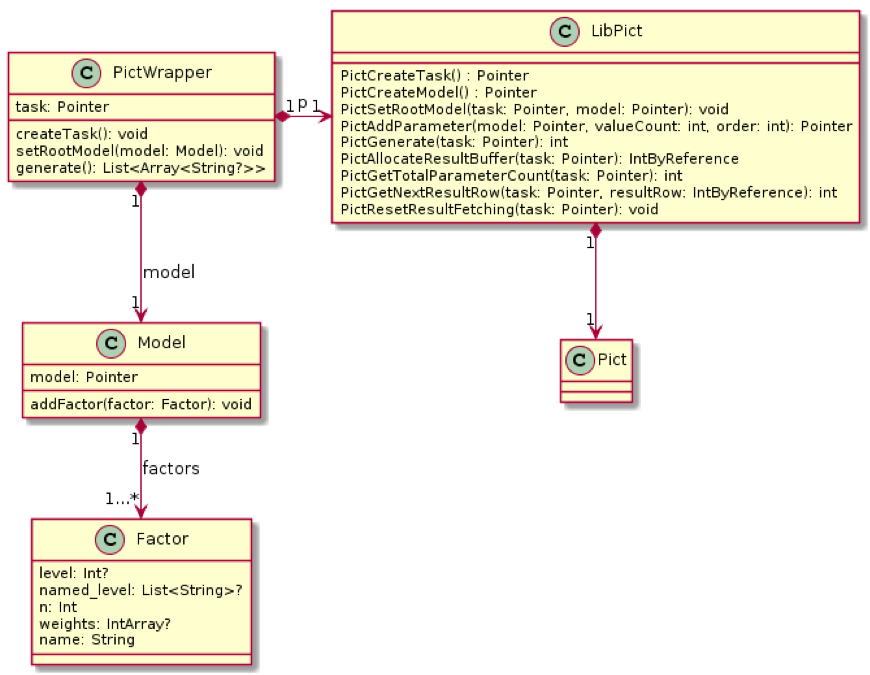
\includegraphics[keepaspectratio, width=160mm]{figs/pict4java_class}
  \caption{pict4javaのクラス図}
  \label{fig:pict4javaClass}
\end{figure}

\newcommand{\PictAddParameter}{\texttt{PictAddParameter}}
\newcommand{\PictGenerate}{\texttt{PictGenerate}}
\newcommand{\PictGetNextResultRow}{\texttt{PictGetNextResultRow}}
\newcommand{\createTask}{\texttt{createTask}}
\newcommand{\setRootModel}{\texttt{setRootModel}}
\newcommand{\generate}{\texttt{generate}}
\newcommand{\addFactor}{\texttt{addFactor}}
\newcommand{\PictAddParameter}{\texttt{PictAddParameter}}


図\ref{fig:pict4javaClass}に、pict4javaのクラス図を示す。それぞれのクラスの説明を、以下に示す。
\begin{itemize}
  \item クラス\texttt{Pict}\\
        Microsoft社が開発したC++で記述されたPICTライブラリである。
  \item クラス\texttt{LibPict}\\
        JNAを用いてJavaで記述したPICTライブラリのインタフェースである。
        メソッド名はすべてPICTライブラリの持つ関数名と同じである。\\
        主に使用するPICTの関数を、以下に示す。
        \begin{description}
          \item[PictAddParameter()] PICTへの因子と水準の登録
          \item[PictGenerate()] 組合せデータの生成
          \item[PictGetNextResultRow()] 生成データの取得
        \end{description}
  \item クラス\texttt{PictWrapper}\\
        PICTを操作するためのクラスである。Kotlin\cite{kotlin}で記述する。以下の機能を持つ。
        \begin{description}
          \item[createTask()] Taskの生成と初期化をする。
                Taskは、PICTの組合せ生成処理の最小単位である。
                PICTライブラリにおけるPictCreateTaskに相当する。
          \item[setRootModel()] TaskにModelの登録をする。
                Modelは因子の集合である。
                PICTライブラリにおけるPictSetRootModelに相当する。
          \item[generate()] ペアワイズ法を適用した組合せの生成をする。
                PICTライブラリにおけるPictGenerateに相当する。
        \end{description}
  \item クラス\texttt{Model}\\
        因子の集合を保持するためのクラスである。Kotlinで記述する。
        \begin{description}
          \item[コンストラクタ()] PICTライブラリにおけるModelを生成する。PictCreateModelに相当する。
          \item[addFactor()] 因子(Factor)をModelに登録する。PICTライブラリにおけるPictAddParameterに相当する。
        \end{description}
  \item クラス\texttt{Factor}
        \begin{description}
          \item[\texttt{level}] 水準
          \item[\texttt{named\_level}] 因子の取り得る値の集合
          \item[\texttt{n}] 最低限組合せるペア数(デフォルトで2)
          \item[\texttt{weights}] 因子の取り得る値の重みの集合
          \item[\texttt{name}] 因子の名前
        \end{description}
        メンバ変数nの値を変えることによって、その因子については、n個の組合せを網羅する入力データを作成できる。
\end{itemize}

\subsection{pict4javaの組込み}
\begin{figure}[tp]
  \centering
  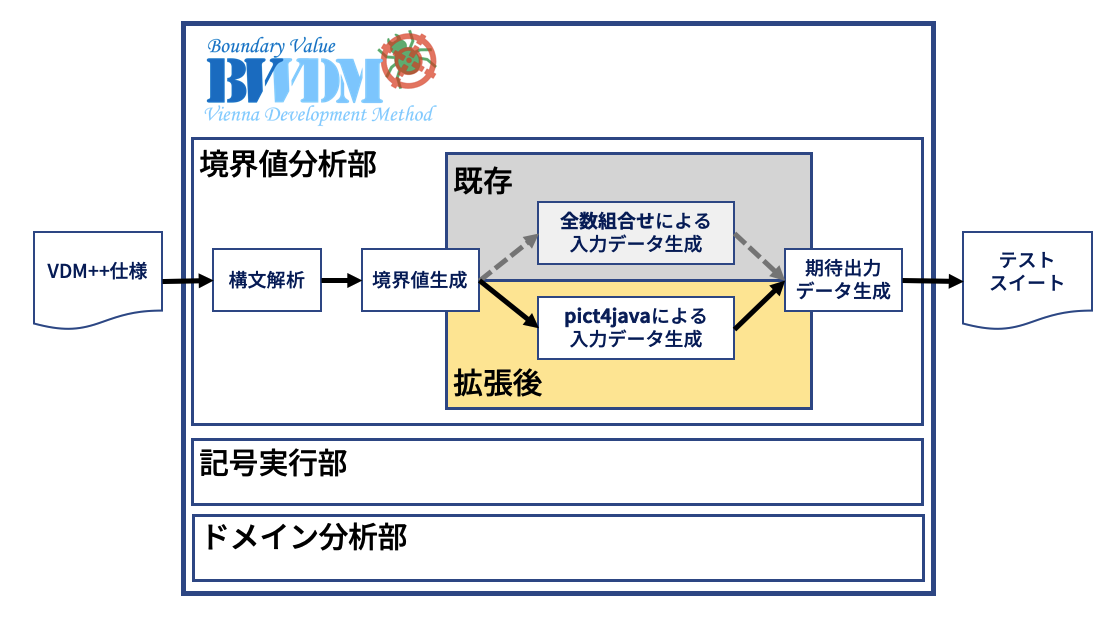
\includegraphics[keepaspectratio, width=160mm]{figs/pict4java_embed}
  \caption{\ref{sec:extendPairwise}節で拡張するBWDMの構造}
  \label{fig:pict4javaEmbed}
\end{figure}

本稿で拡張したBWDMの処理の流れを、図\ref{fig:pict4javaEmbed}に示す。
境界値分析部ではまず、テストケースの入力データとして、VDM++仕様内の引数ごとにおける、不等式、剰余式などに合わせた境界値、及び型の最小値・最大値の境界値を、それぞれ抽出する。
既存のBWDMでは、引数ごとに生成した境界値のすべての組合せを生成し、境界値テストの入力データとしていた。

拡張後のBWDMでは、すべての組合せを生成するのではなく、\ref{sec:create_pict4java}節で述べたpict4javaを用いてペアワイズ法を適用し、入力データ生成を行う。
具体的には、境界値分析で得た因子が取り得る値をpict4javaに入力する。

境界値分析後の境界値データを受けとったpict4javaの入力データ生成アルゴリズムを、以下に示す。
また、このアルゴリズムを用いたpict4javaの処理の流れを、図\ref{fig:pict4java}に示す。

\begin{figure}[tp]
  \centering
  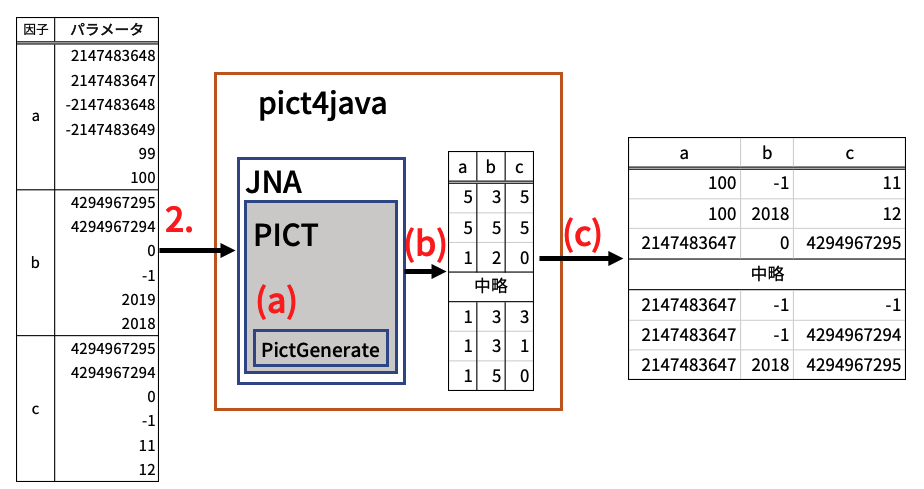
\includegraphics[keepaspectratio, width=160mm]{figs/pict4java}
  \caption{pict4javaの処理の流れ}
  \label{fig:pict4java}
\end{figure}

\begin{enumerate}
  \item 因子と、因子の取り得る値を元に、クラスFactorのインスタンスを因子の数だけ生成する。
  \item クラスModelのaddFactorメソッドを用いて、PictAddParameter関数を呼び出し、PICTに因子と因子ごとの水準を登録する。
  \item\label{enu:pict4java0} クラスPictWrapperのgenerateメソッドを用いて、ペアワイズ法を適用した組合せデータのリストを生成する。
        組合せデータは文字列型の配列のリストである。
        詳細の処理を以下に示す。
        \begin{enumerate}
          \item\label{enu:pict4java1} PictGenerate関数を用いて、PICTにペアワイズ法を適用した組合せデータを生成させる。
          \item\label{enu:pict4java2} PictGetNextResultRow関数を用いて(a)で生成した組合せデータを1件取得する。取得したデータは、因子が取り得るパラメータ群のインデックスとなる。因子の数だけ(b)の処理を繰り返す。
          \item (b)で取得したデータのインデックスに該当するパラメータを用いて、組合せデータのリストを生成する。
        \end{enumerate}
  \item \ref{enu:pict4java0}.で生成したリストを、pict4javaの出力データとする。
\end{enumerate}

\section{ドメイン分析テストの適用による複数変数を含む条件式を含む関数のテストケース生成}\label{sec:extendDomain}

本研究で拡張したBWDMの処理の流れを、図\ref{fig:bwdm_structure}に示す。
既存のBWDMでは、入力したVDM++仕様を構文解析し、その結果を、境界値分析部と記号実行部に渡し、テストケースにおける入力データを生成する。

拡張したBWDMでは、境界値分析部、記号実行部に加えて、ドメイン分析部を追加した。
ドメイン分析部では、\ref{sec:define}節で記述した、inポイント、outポイント、onポイント、offポイントを生成する。
また、複数の変数が条件式に含まれるVDM++仕様の解析に対応できるように、構文解析部を一部修正した。
さらに、ドメインテストに必要な、正常系判定値、着目条件式、そして着目変数の情報をテストケースに含めるために、テストケース生成部において、ドメインテストによるテストケースを出力する際は、正常系判定値、着目条件式、着目変数の情報も出力する処理を追加した。

\begin{figure*}[t]
  \begin{center}
    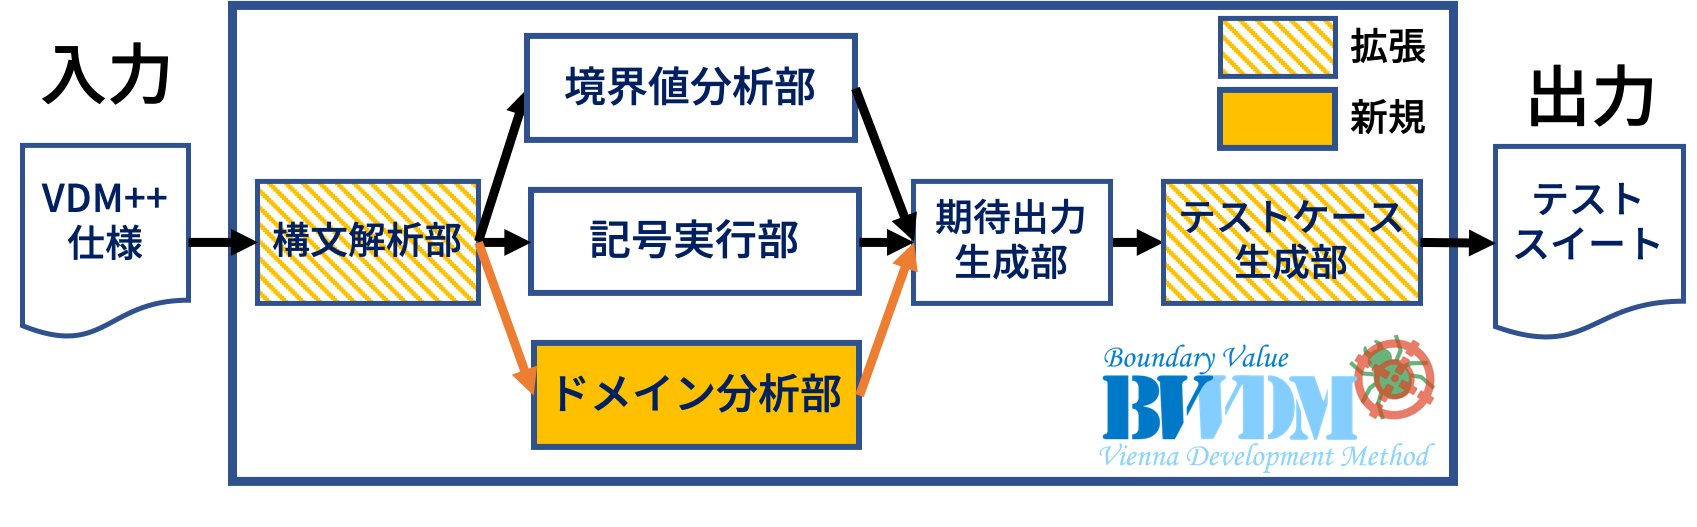
\includegraphics[keepaspectratio, width=160mm]{figs/bwdm_structure.png}
    \caption{\ref{sec:extendPairwise}節で拡張するBWDMの構造}
    \label{fig:bwdm_structure}
  \end{center}
\end{figure*}

\subsection{構文解析部}
% BWDMの構文解析は、Nickらの開発したVDM構文解析ツールVDMJを用いて実現している\cite{vdmj}。
既存のBWDMは、各条件式の左辺、または、右辺に複数の変数を含む場合、エラーを出力してしまう(\ref{sec:bwdm_problem}節)。
したがって、if条件式の左辺と右辺の式を構文解析し、条件式内の変数を抽出することによって、左辺、または、右辺に複数の変数が条件式に含まれるVDM++仕様の構文解析を可能とした。

\subsection{ドメイン分析部}\label{cha:DomainAnalyzer}
拡張したBWDMはドメイン分析テストにおける、onポイント、offポイント、inポイント、outポイントを生成するために、ドメイン分析部を持つ。
各ポイントは、テストケースの入力データであり、引数名と値のタプルの配列を保持している。
各ポイントの生成については、\ref{cha:create_point}節にて説明する。

\begin{figure*}[t]
  \begin{center}
    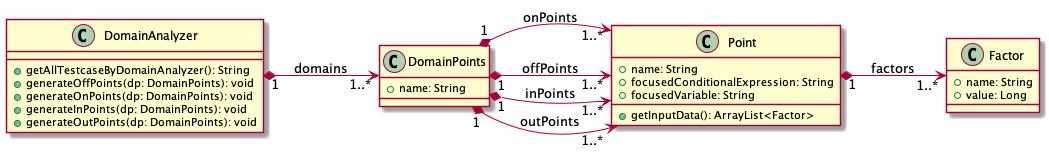
\includegraphics[keepaspectratio, width=160mm]{figs/DomainAnalyzer.png}
    \caption{ドメイン分析部のクラス図}
    \label{fig:class_DomainAnalyzer}
  \end{center}
\end{figure*}

作成したドメイン分析部のクラス図を、図\ref{fig:class_DomainAnalyzer}に示す。
各クラスの詳細を、以下に示す。

\begin{itemize}
  \item
        Factorクラスは、引数の情報を持つクラスである。変数名(name)と値(value)を保持する。
  \item
        Pointクラスは、テストケースの入力データの情報を持つクラスである。テストケース名(name)、そのポイントが着目条件式(forcusedConditionalExpression)、そのポイントの着目変数(forcusedVariable)、そして複数のFactor(factors)を保持する。
  \item
        DomainPointsクラスは、ドメインの情報を持つクラスである。期待出力(name)、onポイントの集合(onPoints)、offポイントの集合(offPoints)、inポイント(inPoints)、outポイントの集合(outPoints)を保持する。
  \item
        DomainAnalyzerクラスは、ドメイン分析を行うクラスである。ドメインの集合(domains)を保持している。
        また、onポイント、offポイント、inポイント、outポイントを生成する機能(generateXXPointsメソッド)、および、各ドメインの各ポイントを、期待出力生成部に入力できるデータ構造として抽出する機能(getAllTestCaseByDomainAnalyzerメソッド)を持つ。

\end{itemize}

\subsection{各ポイントの生成手法の提案と適用}\label{cha:create_point}
拡張したBWDMは、入力する仕様のドメインごとに、onポイント、offポイント、inポイント、outポイントを生成する。

各ポイントを満たす変数の値を求めるために、SMTソルバ(Satisfiable Modulo Theories)\cite{sat}を利用する。
充足可能性問題(SAT)を解くアルゴリズムを実装したソフトウェアをSATソルバと呼び、SATソルバを算術演算に対応させたソフトウェアをSMTソルバと呼ぶ。
幅広く知られているSMTソルバの1つに、Microsoft Researchが開発を進めているZ3\cite{z3}がある。
Z3は、C、C++、Java、Pythonなどのプログラミング言語から利用できるAPIを提供する。
拡張したBWDMは、このZ3を利用し、条件式を満たす入力値を生成する。

各ポイントの生成方法を、以下に示す。

\subsubsection{onポイント}
onポイントは、着目条件式のTBである。ドメインを決定づける条件式に付き1つ生成し、他のonポイントと重複してはならない。
ドメインに関わる条件式の数だけ以下の手順を繰り返し、各条件式に着目したonポイントを生成する。
\begin{enumerate}
  \item\label{enu:onpoint_2} もし、着目条件式の比較演算子が、“$>=$”、または、“$<=$”である場合、“=”に置き換える。“$>$”である場合、“=”で置き換え、右辺を“+1”する。“$<$”である場合、“=”で置き換え、左辺を“+1”する。
  \item\label{enu:onpoint_1} \ref{enu:onpoint_2}.で修正した条件式と、その他の条件式をZ3に入力し、解(引数と値のタプルの集合)を求める。解が求まらなかった場合、現在の着目条件式におけるonポイントが存在しないため、生成を行わずに次の着目条件式のonポイントの生成を行う。
  \item 配列onPoints(\ref{cha:DomainAnalyzer}節)を参照し、他のonポイントと値が重なるかどうかを判定する。
        \begin{enumerate}
          \item 重なっている場合、条件式に、”重なっている変数 $!=$ 重なった値“という条件式を加え、\ref{enu:onpoint_1}.に戻る。
          \item 重なっていない場合、解を元に、Pointインスタンスを作り(\ref{cha:DomainAnalyzer}節)、メンバforcusedConditionalExpressionには、着目条件式を格納する。作成したインスタンスを配列onPointsに格納する。
        \end{enumerate}
\end{enumerate}

\subsubsection{offポイント}
offポイントは、着目するonポイントに隣接し、TBでない値である。onポイントに付き複数(着目条件式に含まれる変数 $*$ 2)個存在する。
配列onPoints(\ref{cha:DomainAnalyzer}節参照)を参照し、onポイントの数だけ以下の手順を繰り返し、onポイントに着目したoffポイントを生成する。
\begin{enumerate}
  \item\label{enu:offpoint_2} 着目するonポイントのメンバforcusedConditionalExpressionを参照し、着目するonポイントがどの条件式に着目していたかを保持する。
  \item \ref{enu:offpoint_2}.の条件式から、引数を抽出する。抽出した引数の数だけ以下を繰り返す。
        \begin{enumerate}
          \item 以下の処理を2回繰り返す。1回目は“N=$-$1”と定義し、2回目は“N=1”と定義する。
                \begin{enumerate}
                  \item\label{enu:offpoint_3} 着目するonポイントインスタンスをコピーする。
                  \item\label{enu:offpoint_1} i.でコピーしたPointインスタンスのメンバ配列factorsから、“Factor.name == 引数名”となるFactorインスタンスを検索する。
                  \item ii.で検索して見つかったFactorインスタンスのメンバvalueを“+N”する。
                  \item PointインスタンスのメンバforcusedVariableに引数名を格納する。
                  \item Pointインスタンスを配列offPoints(\ref{cha:DomainAnalyzer}節)に格納する。
                \end{enumerate}
        \end{enumerate}
\end{enumerate}

\subsubsection{inポイント}
in ポイントは、ドメインを決定づけるすべての条件式を満たす値である。ドメインに付き1つ生成し、他のonポイント、offポイントと重複してはならない。
以下の手順を行い、inポイントを生成する。
\begin{enumerate}
  \item\label{enu:inpoint_2} もし、条件式の比較演算子が、“$>=$”である場合、“$>$”で置き換える。“$<=$”である場合、“$<$”で置き換える。これを、すべての条件式に対して行う。
  \item\label{enu:inpoint_1} \ref{enu:inpoint_2}.で修正した条件式をZ3に入力し、解(引数と値のタプルの集合)を求める。解が求まらなかった場合、inポイントが存在しないため、生成を行わない。
  \item 配列onPointsと配列offPoints(\ref{cha:DomainAnalyzer}節)を参照し、他のonポイント、offポイントと値が重なるかどうかを判定する。
        \begin{enumerate}
          \item 重なっている場合、条件式に、”重なっている変数 $!=$ 重なった値“という条件式を加え、\ref{enu:inpoint_1}.に戻る。
          \item 重なっていない場合、解を元に、Pointインスタンスを作り(\ref{cha:DomainAnalyzer}節)、配列inPointsに格納する。
        \end{enumerate}
\end{enumerate}

\subsubsection{outポイント}
outポイントは、着目条件式のみを満たさない値である。ドメインを決定づける条件式に付き1つ生成し、他のoffポイントと重複してはならない、
ドメインに関わる条件式の数だけ以下の手順を繰り返し、各条件式に着目したoutポイントを生成する。
\begin{enumerate}
  \item\label{enu:outpoint_2} 着目条件式を“$!$(着目条件式)”に置き換え、否定する。
  \item\label{enu:outpoint_1} \ref{enu:outpoint_2}.で否定した条件式と、その他の条件式をZ3に入力し、解(引数と値のタプルの集合)を求める。解が求まらなかった場合、現在の着目条件式におけるoutポイントが存在しないため、生成を行わずに次の着目条件式のoutポイントの生成を行う。
  \item 配列onPointsと配列offPoints(\ref{cha:DomainAnalyzer}節)を参照し、他のonポイント、offポイントと値が重なるかどうかを判定する。
        \begin{enumerate}
          \item 重なっている場合、条件式に、”重なっている変数 $!=$ 重なった値“という条件式を加え、\ref{enu:outpoint_1}.に戻る。
          \item 重なっていない場合、解を元に、Pointインスタンスを作り(\ref{cha:DomainAnalyzer}節)、メンバforcusedConditionalExpressionには、着目条件式を格納する。作成したインスタンスを配列outPointsに格納する。
        \end{enumerate}
\end{enumerate}

\subsection{テストケースの生成}
\begin{figure}[tp]
  \centering
  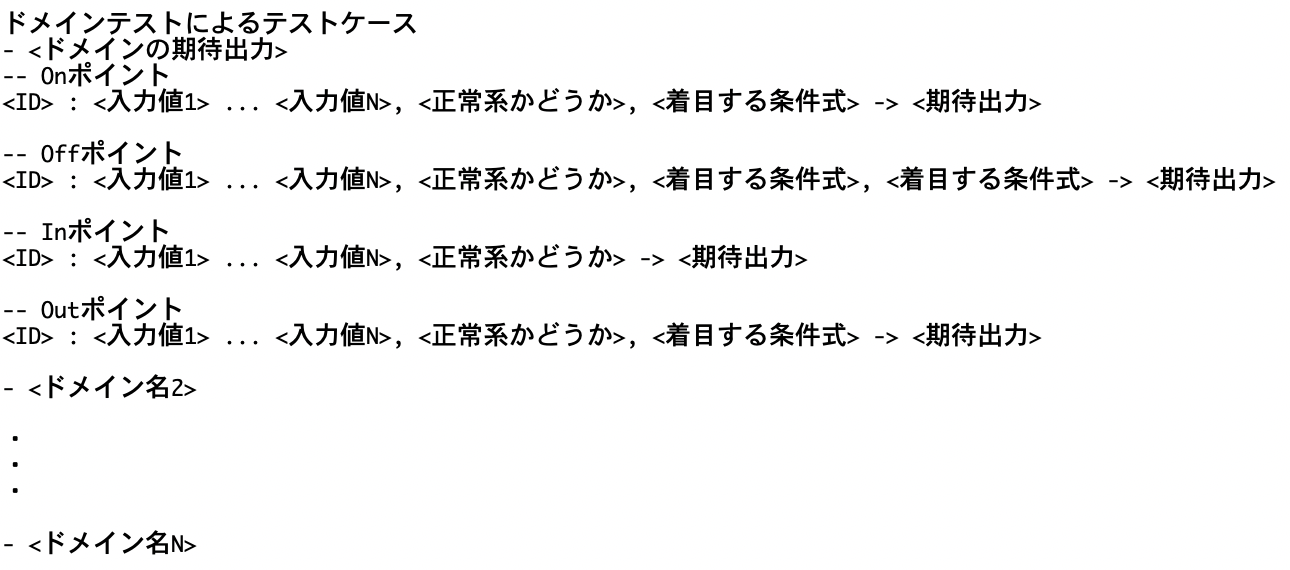
\includegraphics[keepaspectratio, width=160mm]{figs/dmin_output_format}
  \caption{ドメイン分析テストのためのテストケースの出力フォーマット}
  \label{fig:dmin_output_format}
\end{figure}

既存のBWDMは、期待出力生成部において、入力データを元に期待出力を生成する機能を持つ。DomainAnalyzerクラス(\ref{cha:DomainAnalyzer}節参照)のgetAllTestCaseByDomainAnalyzerメソッドを呼び出すことにより、\ref{cha:create_point}節で生成した各ドメインの各ポイントを、期待出力生成部に入力できるデータ構造として抽出することができる。
そのため、既存のBWDMの期待出力生成部をそのまま用いて、期待出力生成とテストケース生成は可能である。
拡張したBWDMでは、各ドメインの各ポイントのテストケースを出力する。

しかし、既存のBWDMのテストケース生成部には、ドメインテストに必要な、正常系判定値、着目条件式、そして着目変数の情報を出力テストケースに加える処理が存在しない。
これに対応するため、テストケース生成部において、ドメインテストによるテストケースを出力する際、正常系判定値、着目条件式、着目変数の情報についても出力する処理を追加した。
着目条件式の出力には、PointクラスのメンバforcusedConditionalExpressionを参照する。
offポイントの場合、着目変数の出力を行う。出力には、PointクラスのメンバforcusedVariableを参照する。
正常系判定値は、出力するテストケースの期待出力と、ドメインの期待出力(DomainPoints.name)を比較して判断する。
等しければ、“正常系”と出力する。等しくなければ“非正常系”と出力する。

出力テストケースのフォーマットを、図\ref{fig:dmin_output_format}に示す。$<$と$>$で囲まれている部分を、それぞれの情報で置き換える。

\section{複数の定義への対応}\label{sec:extendMultiple}
\begin{figure}[tp]
  \centering
  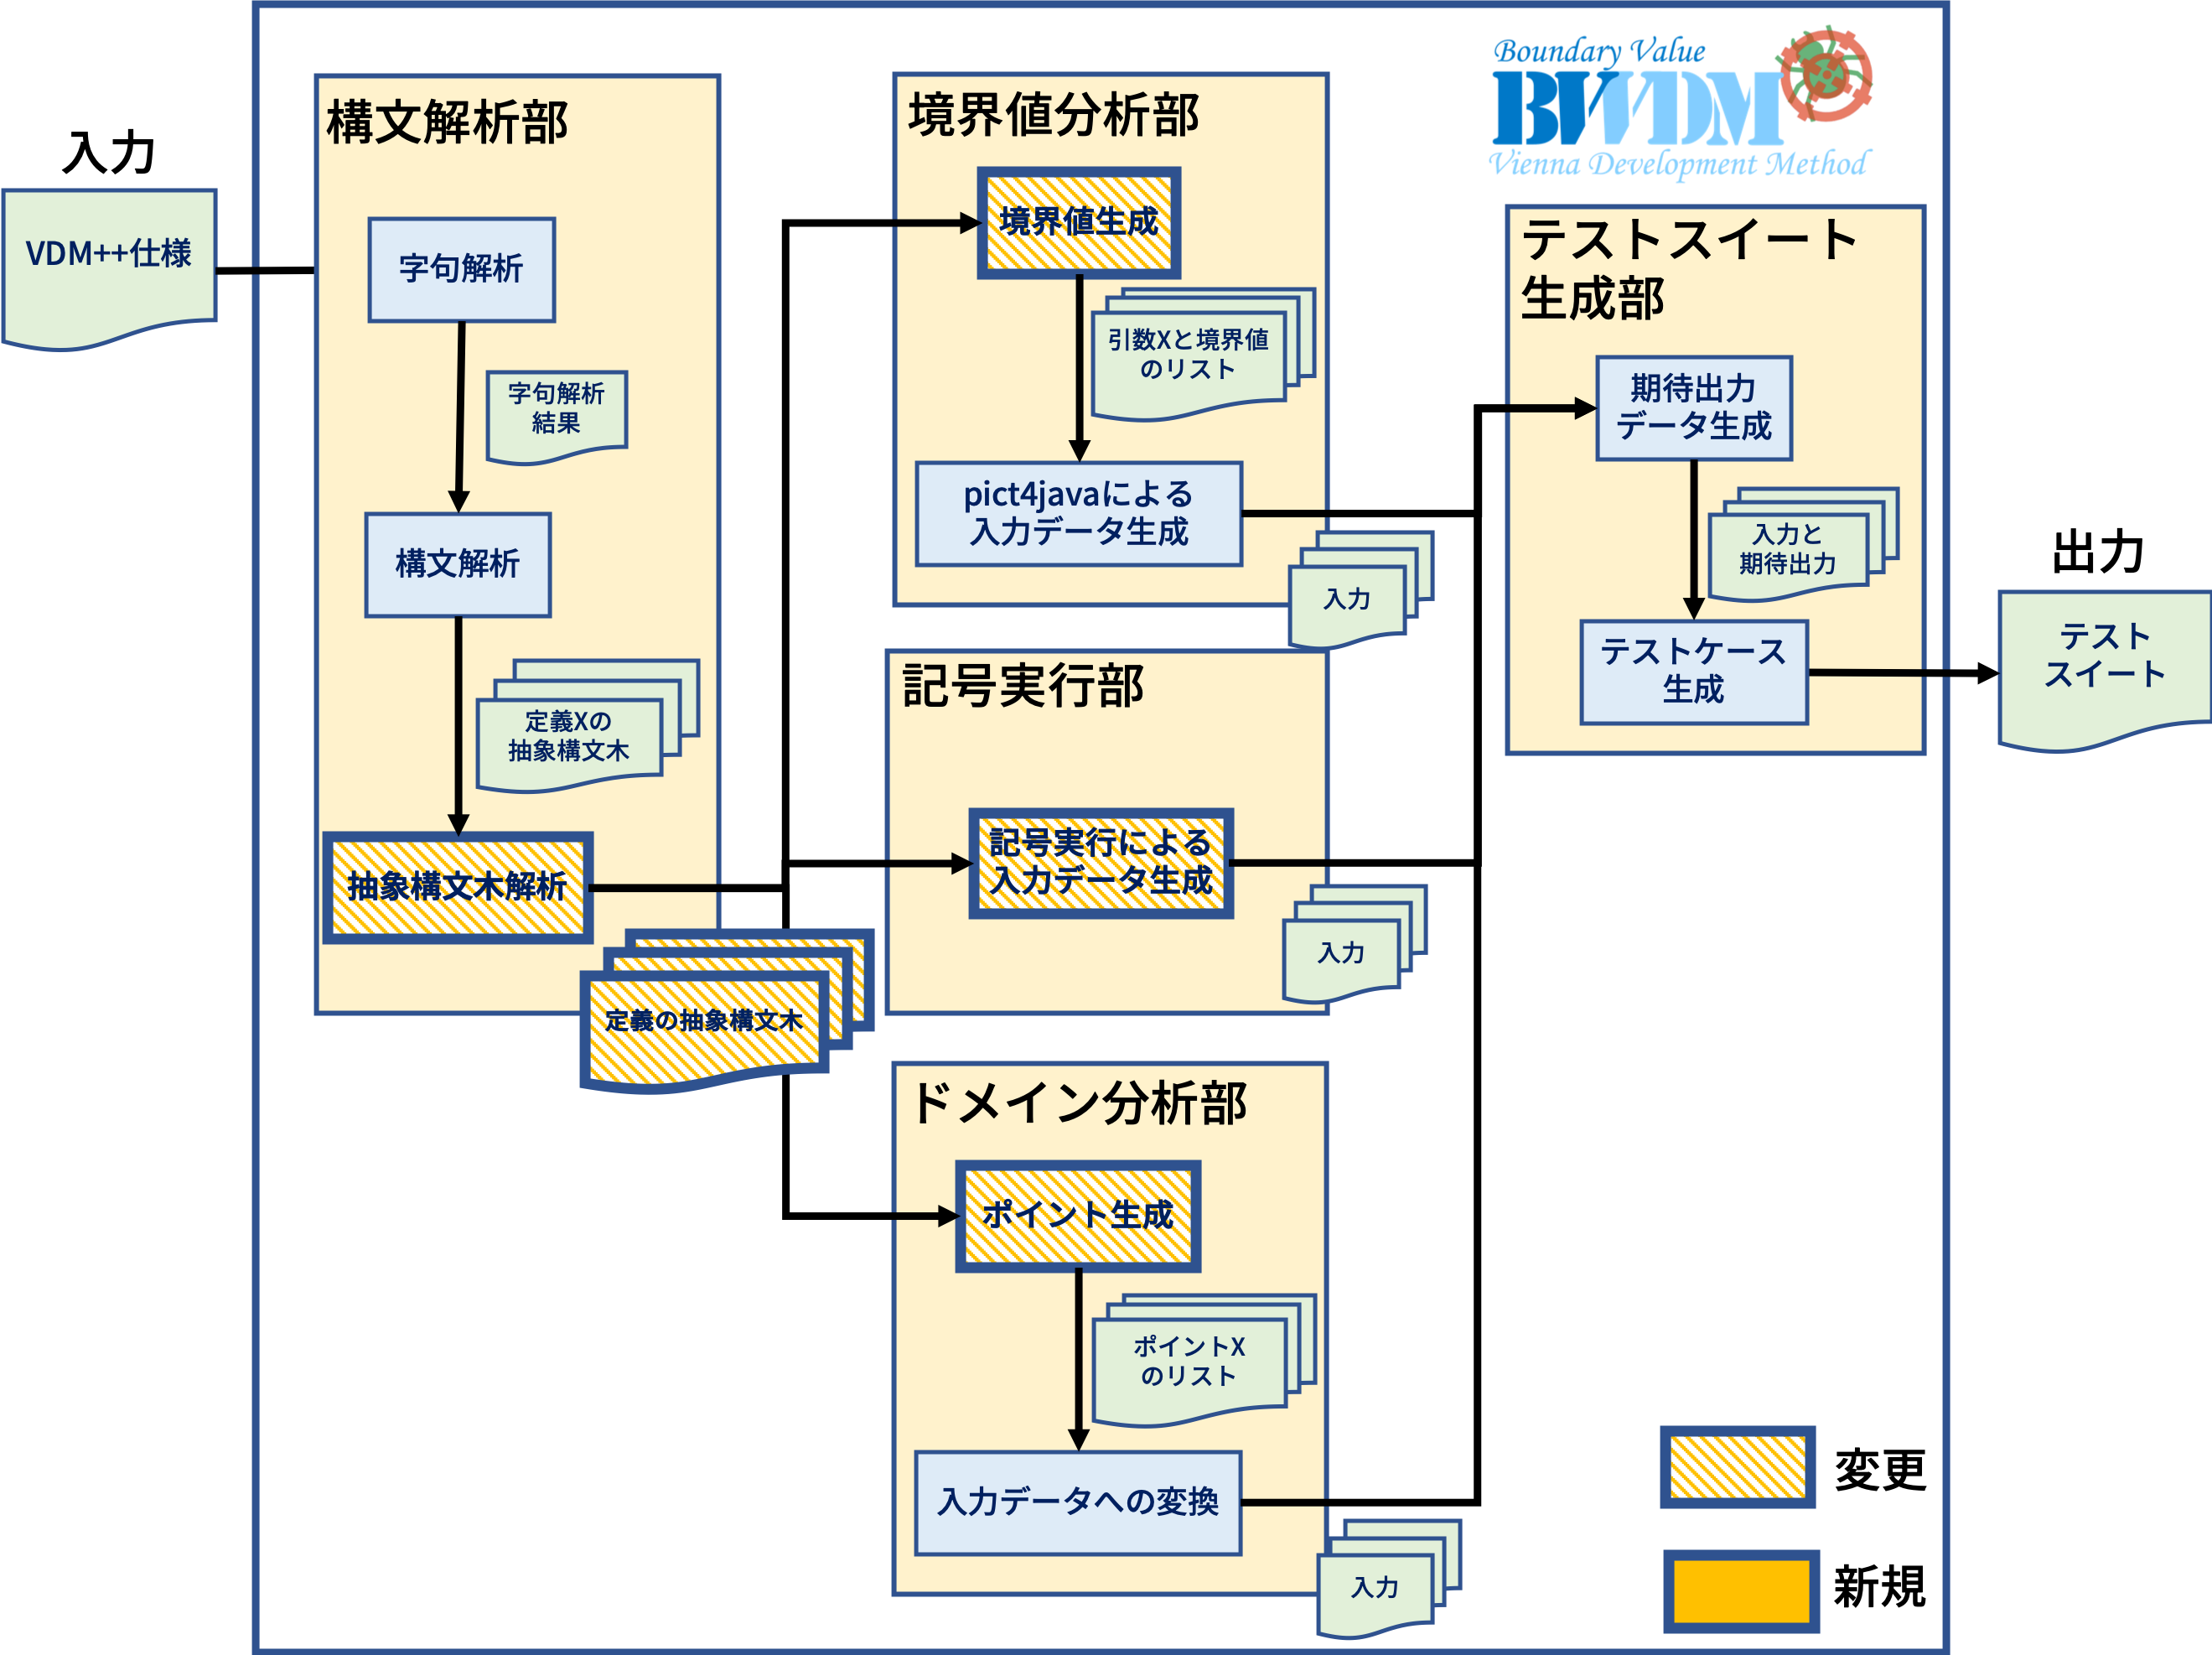
\includegraphics[keepaspectratio, width=160mm]{figs/multi_bwdm_structure}
  \caption{\ref{sec:extendMultiple}節で拡張するBWDMの構造}
  \label{fig:multi_bwdm_structure}
\end{figure}

本研究で拡張したBWDMの処理の流れを、図\ref{fig:multi_bwdm_structure}に示す。
既存のBWDMでは、入力したVDM++仕様を構文解析部に入力し、字句解析、構文解析、抽象構文木解析を行い、最後に定義された定義の抽象構文木を抽出する。

拡張したBWDMでは、\ref{sec:probrem_value}節と\ref{sec:probrem_operation}節で述べた、関数定義以外の定義に対応していないという問題を解決するために、抽象クラスDefinition、クラスFunctionDefinition、クラスOperationDefinitionを新規に作成し、追加した。
また、\ref{sec:probrem_only_function}節で述べた、単一の関数しかテストケース生成できないという問題を解決するため、および、新規に作成したクラスに対応するために、構文解析部の抽象構文木解析処理を一部修正した。

\subsection{定義クラス群の作成}\label{sec:create_definition}
\begin{figure}[tp]
  \centering
  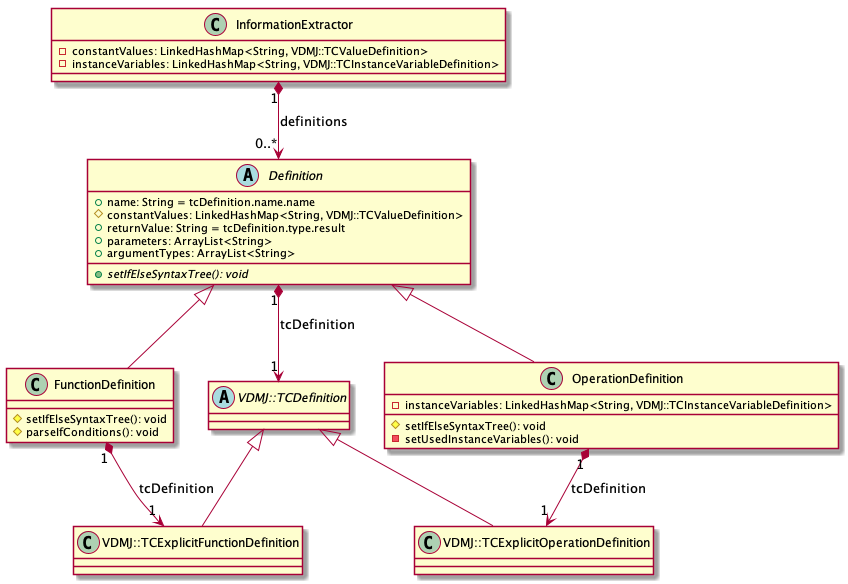
\includegraphics[keepaspectratio, width=160mm]{figs/Definition_class_diagram}
  \caption{Definitionクラス関係のクラス図}
  \label{fig:definition_class}
\end{figure}

関数定義以外の定義に対応するために、抽象クラスDefinition、クラスFunctionDefinition、クラスOperationDefinitionを作成した。
これらの、定義クラス群の関係を、図\ref{fig:definition_class}に示す。
図中にある、VDMJパッケージのクラスはVDMJであらかじめ用意されているクラス(\ref{cha:vdmj}節)である。

それ以外のクラスの説明を以下に示す。

\begin{itemize}
  \item 抽象クラスDefinition\\
        テストケース生成を行う定義を表す抽象クラスである。TCDefinition型のオブジェクトを元に、if-then-else式から木構造を生成\todo{立山さんの修論参照}する。以下のフィールドとメソッドを持つ。
        \begin{description}
          \item[name] 定義の名前
          \item[constantValues] 定数定義の集合
          \item[returnType] 返値の型
          \item[argumentTypes] 引数の型の集合
          \item[parameters] 仮引数名の集合
          \item[setIfElseSyntaxTree()] if-then-else式から木構造を生成する抽象メソッド
          \item[createIfCondition()] if-then-else式を構文解析する
        \end{description}

  \item クラスFunctionDefinition\\
        テストケース生成を行う関数を表すクラスである。\TCExplicitFunctionDefinition{}型のオブジェクトを元に、if-then-else式から木構造を生成する。以下のフィールドとメソッドを持つ。
        \begin{description}
          \item[setIfElseSyntaxTree()] if-then-else式から木構造を生成する。インスタンス生成時にコンストラクタから呼び出される
        \end{description}

  \item クラスOperationDefinition\\
        テストケース生成を行う操作を表すクラスである。TCExplicitOperationDefinition型のオブジェクトを元に、if-then-else式から木構造を生成する。以下のフィールドとメソッドを持つ。
        \begin{description}
          \item[instanceVariables] インスタンス変数定義の集合
          \item[setUsesInstanceVariables()] if-then-else木構造内で使用されるインスタンス変数をargumentTypesとparametersに追加する
          \item[setIfElseSyntaxTree()] if-then-else式から木構造を生成する。インスタンス生成時にコンストラクタから呼び出される
        \end{description}

  \item クラスInformationExtractor\\
        抽象構文木解析処理を行うクラスである。
        構文解析処理から受け取った、定義を表す抽象構文木の集合から、定義クラスの集合を生成する。
        \todo{既存のBWDMにも存在することを明記したほうが良いかも}
        \begin{description}
          \item[constantValues] 定数定義の集合
          \item[instanceVariables] インスタンス変数定義の集合
        \end{description}

\end{itemize}

\subsection{抽象構文木解析処理の修正}

\begin{comment}
\begin{figure}[tp]
  \centering
  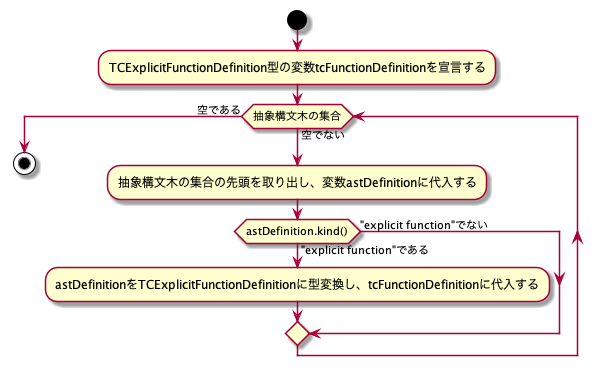
\includegraphics[keepaspectratio, width=160mm]{figs/ExistAstAnalysis}
  \caption{既存のBWDMの抽象構文木解析処理}
  \label{fig:ExistAstAnalysis}
\end{figure}
\end{comment}

既存のBWDMでは、図\ref{fig:multi_bwdm_structure}の構文解析処理で定義ごとの抽象構文木を生成し、それらを抽象構文木解析処理に渡す。
抽象構文木解析処理では、受け取った抽象構文木の集合から、関数定義であるものだけを抽出する。
受け取る抽象構文木の集合は、\ref{sec:create_definition}節で示した抽象クラスTCDefinitionを継承したクラスの集合である。
既存のBWDMの抽象構文木解析処理を以下に示す。
以下の処理はInformationExtractorクラスにて行う。

%既存のBWDMの抽象構文木解析処理を図\ref{fig:ExistAstAnalysis}に示す。

\begin{enumerate}
  \item \TCExplicitFunctionDefinition{}型の変数\tcFunctionDefinition{}を宣言する。
  \item\label{enu:checkAstIsNull} 構文解析処理で生成した抽象構文木の集合が空であるか確認する。空でない場合、\ref{enu:ast_not_null}へ進む。
        空である場合、変数\tcFunctionDefinition{}を構文木解析処理の出力とし、処理を終了する。
  \item\label{enu:ast_not_null} 抽象構文木の集合の先頭を取り出し、変数\astDefinition{}に格納する。
  \item\label{enu:ast_kind} \astDefinition{}.kind()を実行し、定義の種類を取得する。
  \item \ref{enu:ast_kind}で取得した定義の種類(表\ref{tab:vdmj_definition_name})が"explicit function"であるか確認する。
        "explicit function"である場合、\ref{enu:ast_dainyu}へ進む。
        "explicit function"でない場合、\ref{enu:checkAstIsNull}へ進む。
  \item\label{enu:ast_dainyu} 変数\astDefinition{}を\TCExplicitFunctionDefinition{}に型変換し、変数\tcFunctionDefinition{}に代入する。
  \item \ref{enu:checkAstIsNull}に進む。
\end{enumerate}


拡張したBWDMでは、抽象構文木解析処理にて、受け取った抽象構文木を、\ref{sec:create_definition}節で作成した定義クラス群に変換し、連想配列に格納している。
拡張したBWDMの抽象構文木解析処理を以下に示す。以下の処理はInformationExtractorクラスにて行う。

\begin{enumerate}
  \item FunctionDefinition型の連想配列explicitFunctionsをインスタンス化する。
  \item OperationDefinition型の連想配列explicitOperationsをインスタンス化する。
  \item TCValueDefinition型の連想配列constantValuesをインスタンス化する。
  \item TCInstanceVariableDefinition型の連想配列instanceVariablesをインスタンス化する。
  \item\label{enu:checkAstIsNull2} 構文解析処理で生成した抽象構文木の集合が空であるか確認する。空でない場合、\ref{enu:ast_not_null2}へ進む。
        空である場合、連想配列explicitFunctionsと連想配列explicitOperationsを構文木解析処理の出力とし、処理を終了する。
  \item\label{enu:ast_not_null2} 抽象構文木の集合の先頭を取り出し、変数\astDefinition{}に格納する。
  \item\label{enu:ast_kind2} \astDefinition{}.kind()を実行し、抽象構文木の種類を取得する。
  \item \ref{enu:ast_kind2}で取得した抽象構文木の種類を確認し、種類に応じて以下のいずれかを実行する。
        \begin{enumerate}
          \item "explicit function"である場合、関数定義なので、以下を実行する。
                \begin{enumerate}
                  \item 変数\astDefinition{}を\TCExplicitFunctionDefinition{}に型変換し、クラスFunctionDefinitionに渡し、インスタンス化する。
                  \item インスタンス化したクラスFunctionDefinitionを、連想配列explicitFunctionsに、キーを定義名(\astDefinition{}.name)として追加する。
                \end{enumerate}
          \item "explicit operation"である場合、操作定義なので、以下を実行する。
                \begin{enumerate}
                  \item 変数\astDefinition{}をTCExplicitOperationDefinitionに型変換し、クラスOperationDefinitionに渡し、インスタンス化する。
                  \item インスタンス化したクラスOperationDefinitionを、連想配列explicitOperationsに、キーを定義名(\astDefinition{}.name)として追加する。
                \end{enumerate}
          \item "value"である場合、定数定義なので、\astDefinition{}をTCValueDefinitionに型変換し、tcValueDefinitionに追加する。
          \item "instance variable"である場合、インスタンス変数定義なので、\astDefinition{}をTCInstanceVariableDefinitionに型変換し、tcInstanceVariableDefinitionに追加する。
          \item (a)、(b)、(c)、(d)のいずれでもない場合、\ref{enu:checkAstIsNull2}へ進む。
        \end{enumerate}
\end{enumerate}

%拡張したBWDMの抽象構文木解析処理を図\ref{fig:ExtendedAstAnalysis}に示す。
\begin{comment}
\begin{figure}[tp]
  \centering
  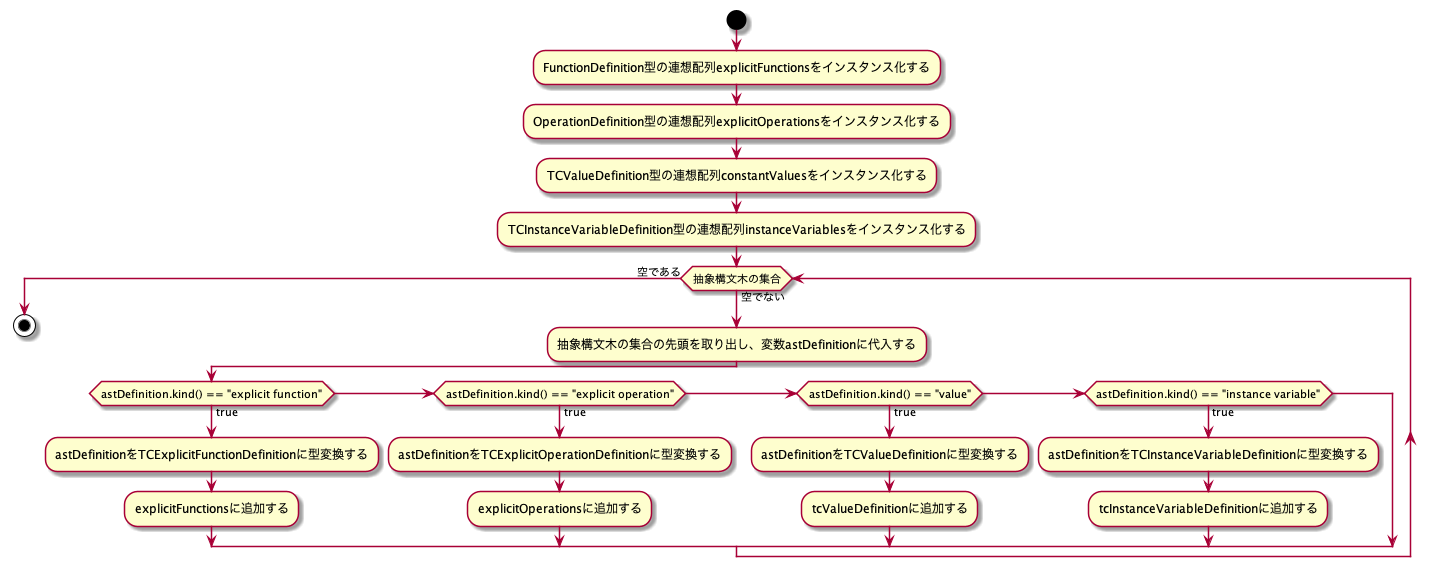
\includegraphics[keepaspectratio, width=160mm]{figs/ExtendedAstAnalysis}
  \caption{拡張したBWDMの抽象構文木解析処理}
  \label{fig:ExtendedAstAnalysis}
\end{figure}
\end{comment}

\subsection{境界値分析部、記号実行部、ドメイン分析部で定義クラス群を入力とするように修正}
既存のBWDMでは、境界値分析部、記号実行部、ドメイン分析部に入力するオブジェクトの型が\TCExplicitFunctionDefinition{}型であった。
したがって、拡張したBWDMでは、\ref{sec:create_definition}節で作成した定義クラス群を境界値分析部、記号実行部、ドメイン分析部に入力できるように修正する。

% 適用例
\chapter{適用例}\label{cha:Indication}
本章では、本研究で拡張したBWDMが正しく動作することを確認する。


\section{因子と水準の組合せ数が大きい仕様}

\lstset{language=}
\noindent\begin{minipage}{\textwidth}
  \begin{lstlisting}[caption=因子が3、水準が(6 6 6)の関数を持つVDM++仕様,label=fig:pict4javaSampleVdm]
class SampleClass
functions

sampleFunction : int*nat*nat -> seq of char
sampleFunction(a, b, c)==
  if(a < 100) then
    if(b > 2018) then
      "aは100未満かつbは2018より大きい"
    else
      "aは100未満かつbは2018以下"
  elseif(c < 12) then
    "aは100以上かつcは12未満"
  else
    "aは100以上かつcは12以上";

end SampleClass
\end{lstlisting}
\end{minipage}

\lstset{language=}
\noindent\begin{minipage}{\textwidth}
  \begin{lstlisting}[caption=コード\ref{fig:pict4javaSampleVdm}の適用結果,label=fig:pict4javaTekiyourei]

関数名 : sampleFunction
引数の型 : a:int b:nat c:nat 
戻り値の型 : seq of (char)
生成テストケース数 : 44件(境界値分析:40/記号実行:4)

各引数の境界値
a : 2147483648 2147483647 -2147483648 -2147483649 99 100 
b : 4294967295 4294967294 0 -1 2019 2018 
c : 4294967295 4294967294 0 -1 11 12 

記号実行情報
戻り値の数 : 4
制約 : b > 2018 and a < 100, 戻り値 : "aは100未満かつbは2018より大きい"
制約 : !( b > 2018 ) and a < 100, 戻り値 : "aは100未満かつbは2018以下"
制約 : c < 12 and !( a < 100 ) , 戻り値 : "aは100以上かつcは12未満"
制約 : !( c < 12 ) and !( a < 100 ) , 戻り値 : "aは100以上かつcは12以上"

境界値分析によるテストケース(ペアワイズ法適用)
No.1 : 100 4294967295 -1 -> Undefined Action
No.2 : 2147483648 2019 -1 -> Undefined Action
No.3 : 100 2019 11 -> "aは100以上かつcは12未満"
No.4 : 2147483648 2018 4294967294 -> Undefined Action
No.5 : 2147483647 -1 4294967294 -> Undefined Action
No.6 : -2147483649 0 0 -> Undefined Action
No.7 : 2147483648 -1 4294967295 -> Undefined Action
No.8 : 100 -1 12 -> Undefined Action
No.9 : -2147483649 2019 12 -> Undefined Action
No.10 : 99 -1 0 -> Undefined Action
No.11 : 99 4294967295 11 -> Undefined Action
No.12 : 99 2019 4294967294 -> "aは100未満かつbは2018より大きい"
No.13 : -2147483648 2018 -1 -> Undefined Action
No.14 : 100 2018 0 -> "aは100以上かつcは12未満"
No.15 : 99 4294967294 -1 -> Undefined Action
No.16 : -2147483649 2018 4294967295 -> Undefined Action
No.17 : 2147483647 4294967295 4294967295 -> Undefined Action
No.18 : 100 0 4294967295 -> Undefined Action
No.19 : 2147483647 0 12 -> "aは100以上かつcは12以上"
No.20 : 99 2018 12 -> "aは100未満かつbは2018以下"
No.21 : -2147483648 4294967294 4294967295 -> Undefined Action
No.22 : 2147483647 4294967294 0 -> "aは100以上かつcは12未満"
No.23 : 99 0 4294967295 -> Undefined Action
No.24 : -2147483649 4294967294 4294967294 -> Undefined Action
No.25 : 2147483647 2019 4294967295 -> Undefined Action
No.26 : -2147483648 0 11 -> "aは100未満かつbは2018以下"
No.27 : 2147483648 4294967294 11 -> Undefined Action
No.28 : 2147483647 -1 -1 -> Undefined Action
No.29 : -2147483649 -1 11 -> Undefined Action
No.30 : 100 4294967294 12 -> "aは100以上かつcは12以上"
No.31 : 2147483648 4294967295 0 -> Undefined Action
No.32 : 100 4294967295 4294967294 -> Undefined Action
No.33 : 2147483647 2018 11 -> "aは100以上かつcは12未満"
No.34 : 2147483648 0 4294967294 -> Undefined Action
No.35 : -2147483648 2019 0 -> "aは100未満かつbは2018より大きい"
No.36 : 2147483648 4294967295 12 -> Undefined Action
No.37 : -2147483648 4294967295 4294967294 -> Undefined Action
No.38 : -2147483648 -1 12 -> Undefined Action
No.39 : -2147483649 0 -1 -> Undefined Action
No.40 : -2147483649 4294967295 0 -> Undefined Action
\end{lstlisting}
\end{minipage}

\ref{sec:extendPairwise}節で拡張したBWDMが正しく動作することを検証するため、拡張したBWDMに因子と水準の組合せ数が大きいVDM++仕様を適用した。
適用例として用いる、因子が3、境界値生成後の水準がそれぞれ(6, 6, 6)の関数のVDM++仕様を、コード\ref{fig:pict4javaSampleVdm}に示す。
適用結果を、コード\ref{fig:pict4javaTekiyourei}に示す。

この適用結果から、既存のBWDMでは$6 \times 6 \times 6 = 216個$生成していたテストケースを、拡張後のBWDMでは40個の生成に抑えており、かつ、40個のテストケースは、2個の因子のペアの組合せをすべて網羅できていることが確認できた。
すなわち、拡張したBWDMが、VDM++仕様から、ペアワイズ法を適用した境界値テストケースを正しく出力できていることが確認できた。


\section{複数変数を含む条件式を用いた仕様}
\begin{figure}[tp]
  \centering
  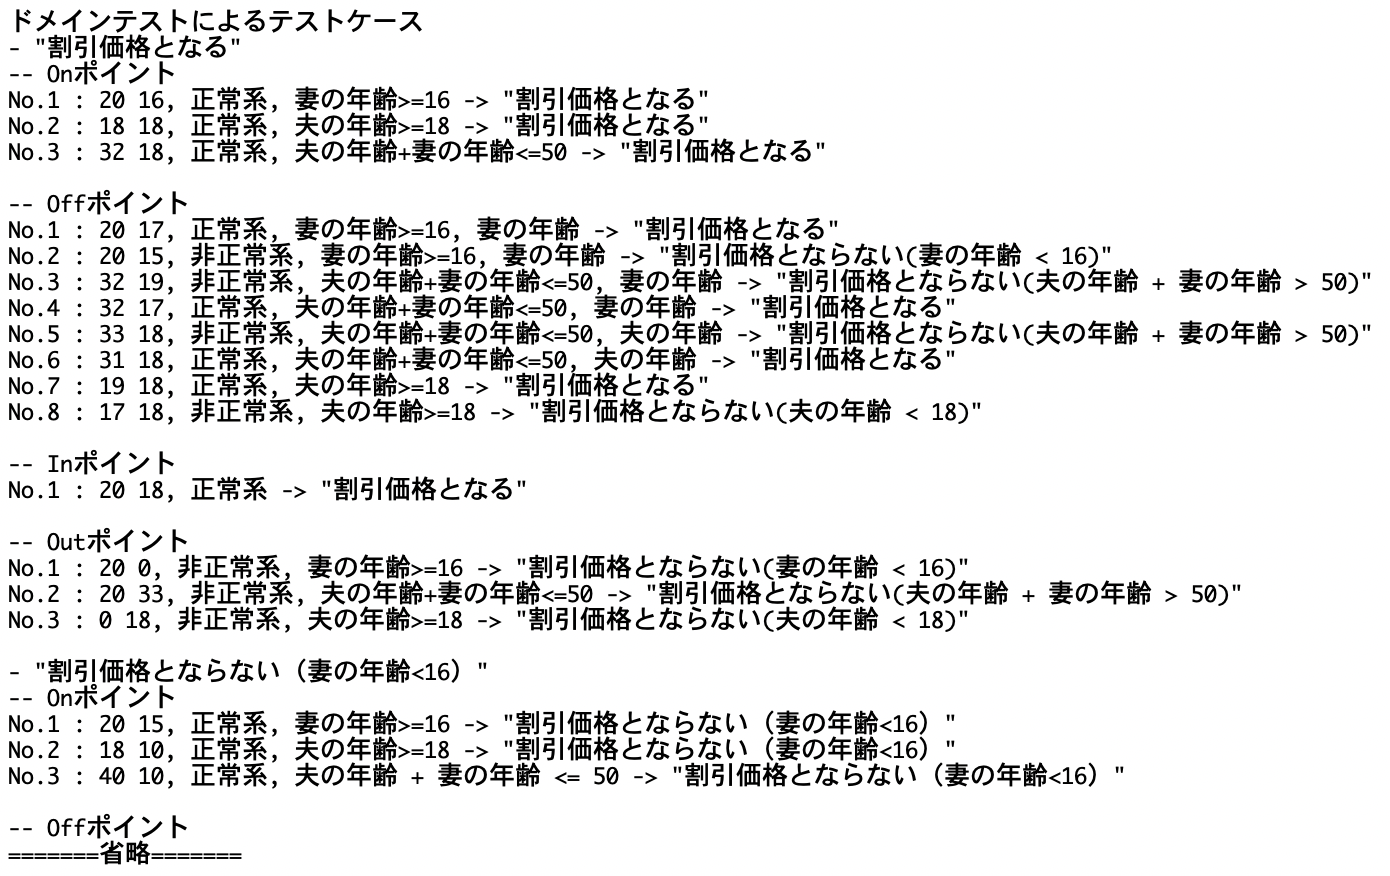
\includegraphics[keepaspectratio, width=160mm]{figs/tekiyourei}
  \caption{遊園地チケット割引機能(コード\ref{fig:vdm_park})のテストケースの一部}
  \label{fig:park_testcase}
\end{figure}

拡張したBWDMに、遊園地チケット割引機能( コード\ref{fig:vdm_park})を入力として適用した結果の一部を、図\ref{fig:park_testcase}に示す。
図\ref{fig:park_testcase}では、“割引価格となる”期待出力以外の3つの期待出力を持つドメイン(“割引価格とならない(妻の年齢 $<$ 16)”、“割引価格とならない(夫の年齢 $<$ 18)”、“割引価格とならない(夫の年齢 + 妻の年齢 $>$ 50)”)のテストケースは省略してある。

“割引価格となる”ドメインの3つのonポイントは、ドメインを決定づける3つの条件式(“夫の年齢 + 妻の年齢 $<=$ 50”、“夫の年齢 $>=$ 18”、“妻の年齢 $>=$ 16”)にそれぞれ着目し、着目条件式のTBが入力となっており、かつ、期待出力と正常系判定値(ポイントの期待出力とドメインの期待出力が一致するかどうか)が適切であることが確認できる。
offポイントは、各onポイントに隣接しており、TBではない値が入力となっており、かつ、着目変数、期待出力、正常系判定値が適切であることが確認できる。
inポイントは、期待出力とドメインの期待出力が一致しており、各条件式のTBでない値が入力となっており、かつ、正常系であることが確認できる。
outポイントは、関係する3つの条件式に着目し、着目条件式のみを否定するTBでない値が入力となっており、かつ、期待出力と正常系判定値が適切であることが確認できる。

また、図\ref{fig:park_testcase}では省略している、“割引価格となる”期待出力以外の期待出力を持つドメイン(“割引価格とならない(妻の年齢 $<$ 16)”、“割引価格とならない(夫の年齢 $<$ 18)”、“割引価格とならない(夫の年齢 + 妻の年齢 $>$ 50)”)に対しても、テストケースが適切に生成できていることを確認した。

したがって、拡張したBWDMは、既存のBWDMの問題点である、条件式内に複数の変数があるVDM++仕様を解析できること、かつ、ドメインテストによるテストケース生成が適切にできることを確認できた。


\section{複数の関数を含む仕様}
拡張したBWDMに、複数の関数を含む仕様(コード\ref{fig:func_multiple})を入力として適用した結果を、コード\ref{fig:extended_func_multiple_result}に示す。
コード\ref{fig:extended_func_multiple_result}では、「成人判定」関数だけでなく、「うるう年判定」関数についてもテストケース生成が適切にできていることが確認できる。

したがって、拡張したBWDMは、既存のBWDMの問題点である、単一の関数しかテストケース生成できないという問題点を解決し、複数の関数のテストケース生成ができることを確認できた。

\lstset{language=}
\noindent\begin{minipage}{\textwidth}
  \begin{lstlisting}[caption=拡張したBWDMにコード\ref{fig:func_multiple}を適用した際の出力,label=fig:extended_func_multiple_result]
関数名 : うるう年判定
引数の型 : 年:int 
戻り値の型 : seq of (char)
生成テストケース数 : 17件(境界値分析:13/記号実行:4)

各引数の境界値
年 : 2147483648 2147483647 -2147483648 -2147483649 3 4 5 99 100 101 399 400 401 

記号実行情報
戻り値の数 : 4
制約 : 年 mod 400 = 0 and 年 mod 100 = 0and 年 mod 4 = 0, 戻り値 : "うるう年"
制約 : !( 年 mod 400 = 0 ) and 年 mod 100 = 0and 年 mod 4 = 0, 戻り値 : "平年"
制約 : !( 年 mod 100 = 0 ) and 年 mod 4 = 0, ��り値 : "うるう年"
制約 : !( 年 mod 4 = 0 ) , 戻り値 : "平年"

境界値分析によるテストケース
No.1 : 2147483648 -> Undefined Action
No.2 : 2147483647 -> "平年"
No.3 : -2147483648 -> "うるう年"
No.4 : -2147483649 -> Undefined Action
No.5 : 3 -> "平年"
No.6 : 4 -> "うるう年"
No.7 : 5 -> "平年"
No.8 : 99 -> "平年"
No.9 : 100 -> "平年"
No.10 : 101 -> "平年"
No.11 : 399 -> "平年"
No.12 : 400 -> "うるう年"
No.13 : 401 -> "平年"

記号実行によるテストケース
No.1 : 400 -> "うるう年"
No.2 : 500 -> "平年"
No.3 : 104 -> "うるう年"
No.4 : 1 -> "平年"

関数名 : 成人判定
引数の型 : 年齢:nat 
戻り値の型 : seq of (char)
生成テストケース数 : 8件(境界値分析:6/記号実行:2)

各引数の境界値
年齢 : 4294967295 4294967294 0 -1 20 21 

記号実行情報
戻り値の数 : 2
制約 : 年齢 <= 20 , 戻り値 : "未成年"
制約 : !( 年齢 <= 20 ) , 戻り値 : "成人"

境界値分析によるテストケース
No.1 : 4294967295 -> Undefined Action
No.2 : 4294967294 -> "成人"
No.3 : 0 -> "未成年"
No.4 : -1 -> Undefined Action
No.5 : 20 -> "未成年"
No.6 : 21 -> "成人"

記号実行によるテストケース
No.1 : 1 -> "未成年"
No.2 : 21 -> "成人"

\end{lstlisting}
\end{minipage}

\section{定数を含む関数を含む仕様}
拡張したBWDMに、定数を含む関数を含む仕様(コード\ref{fig:value_definition})を入力として適用した結果をコード\ref{fig:extended_value_definition_result}に示す。
コード\ref{fig:extended_value_definition_result}では、12行目にて「$数 mod 2 = 0$」となっており、evenを2に正しく変換できていることが確認できる。
また、13行目も同様に確認できる。
また、入力と出力の組合せが正しいことから、テストケース生成が適切にできていることが確認できた。

したがって、拡張したBWDMは、既存のBWDMの問題点である、定数を含む関数を含む仕様のテストケース生成ができないという問題点を解決し、定数を含む関数を含む仕様のテストケース生成ができることを確認できた。

\lstset{language=}
\noindent\begin{minipage}{\textwidth}
  \begin{lstlisting}[caption=拡張したBWDMにコード\ref{fig:func_multiple}を適用した際の出力,label=fig:extended_value_definition_result]

関数名 : 偶数判定
引数の型 : 数:int 
戻り値の型 : seq of (char)
生成テストケース数 : 9件(境界値分析:7/記号実行:2)

各引数の境界値
数 : 2147483648 2147483647 -2147483648 -2147483649 1 2 3 

記号実行情報
戻り値の数 : 2
制約 : 数 mod 2 = 0 , 戻り値 : "偶数"
制約 : !( 数 mod 2 = 0 ) , 戻り値 : "奇数"

境界値分析によるテストケース
No.1 : 2147483648 -> Undefined Action
No.2 : 2147483647 -> "奇数"
No.3 : -2147483648 -> "偶数"
No.4 : -2147483649 -> Undefined Action
No.5 : 1 -> "奇数"
No.6 : 2 -> "偶数"
No.7 : 3 -> "奇数"

記号実行によるテストケース
No.1 : 2 -> "偶数"
No.2 : 1 -> "奇数"

\end{lstlisting}
\end{minipage}

\section{操作定義を含む仕様}
拡張したBWDMに、操作定義を含む仕様(コード\ref{fig:multiple_definition})を入力として適用した結果をコード\ref{fig:extended_multiple_definition}に示す。
コード\ref{fig:extended_multiple_definition}では、インスタンス変数「current\_year」を「うるう年判定」操作の引数としてテストケース生成できていることが確認できる。
また、入力と出力の組合せが正しいことから、適切なテストケース生成ができていることが確認できた。

したがって、拡張したBWDMは、既存のBWDMの問題点である、操作のテストケース生成ができないという問題点を解決し、操作のテストケース生成ができることを確認できた。

\lstset{language=}
\noindent\begin{minipage}{\textwidth}
  \begin{lstlisting}[caption=拡張したBWDMにコード\ref{fig:multiple_definition}を適用した際の出力,label=fig:extended_multiple_definition]

関数名 : うるう年判定
引数の型 : current_year:nat 
戻り値の型 : seq of (char)
生成テストケース数 : 17件(境界値分析:13/記号実行:4)

各引数の境界値
current_year : 4294967295 4294967294 0 -1 3 4 5 99 100 101 399 400 401 

記号実行情報
戻り値の数 : 4
制約 : current_year mod 400 = 0 and current_year mod 100 = 0and current_year mod 4 = 0, 戻り値 : "うるう年"
制約 : !( current_year mod 400 = 0 ) and current_year mod 100 = 0and current_year mod 4 = 0, 戻り値 : "平年"
制約 : !( current_year mod 100 = 0 ) and current_year mod 4 = 0, 戻り値 : "うるう年"
制約 : !( current_year mod 4 = 0 ) , 戻り値 : "平年"

境界値分析によるテストケース
No.1 : 4294967295 -> Undefined Action
No.2 : 4294967294 -> "平年"
No.3 : 0 -> "うるう年"
No.4 : -1 -> Undefined Action
No.5 : 3 -> "平年"
No.6 : 4 -> "うるう年"
No.7 : 5 -> "平年"
No.8 : 99 -> "平年"
No.9 : 100 -> "平年"
No.10 : 101 -> "平年"
No.11 : 399 -> "平年"
No.12 : 400 -> "うるう年"
No.13 : 401 -> "平年"

記号実行によるテストケース
No.1 : 400 -> "うるう年"
No.2 : 100 -> "平年"
No.3 : 4 -> "うるう年"
No.4 : 1 -> "平年"
    
\end{lstlisting}
\end{minipage}

% 考察
\chapter{考察}\label{cha:Evaluation}
本章では、拡張したBWDMを考察する。

\section{評価}
\subsection{膨大な数のテストケースを生成}

\begin{table}[tp]
  \begin{center}
    \caption{因子が7、水準が(6 8 6 8 8 6 6)の関数を持つVDM++仕様の生成結果の比較}
    \label{tab:pict4java_result}
    \begin{tabular}{c|c|c}
                   & 生成テストケース数 & 実行時間(秒) \\
      \hline
      \hline
      既存のBWDM   & 663,552            & 6.767146152  \\ \hline
      拡張したBWDM & 78                 & 0.88973152
    \end{tabular}
  \end{center}
\end{table}

\lstset{language=}
\noindent\begin{minipage}{\textwidth}
  \begin{lstlisting}[caption=因子が7、水準が(6 8 6 8 8 6 6)の関数を持つVDM++仕様,label=fig:pict4javaIndication]
class ProblemClass
functions

problemFunction : nat*nat*nat*nat*nat*nat*nat -$>$ seq of char
  problemFunction(a, b, c, d, e, f, g) ==
    if(a > 4) then
      if(b mod 10 = 3) then
        if(c < 13) then
          if(b > 11) then
            "a>4 and b>11 and c<13"
          else
            if(g < 11) then
              "g<11"
            else
              "a>4 and b>10 and c<13"
        else
          if(d > 10) then
            "d>10"
          else
            if(e < 10) then
              "e<10"
            elseif(f > 10) then
              "f>10"
            else
              "a>4 and b>10 and c>=13"
      else
        "a>4 and b<=10"
    else
      "a<=4";
end ProblemClass
\end{lstlisting}
\end{minipage}

本稿で拡張したBWDMが、既存のBWDMに比べて、テストケース総数を削減できることを確認する。
膨大な数のテストケースを生成するために、因子が7、境界値生成後の水準がそれぞれ(6, 8, 6, 8, 8, 6, 6)の関数を持つVDM++仕様を、既存のBWDMと拡張後のBWDMにそれぞれ適用する。
生成結果の比較を、表\ref{tab:pict4java_result}に示す。
また、適用したVDM++仕様をコード\ref{fig:pict4javaIndication}に示す。
実行環境は、macOS 10.13.6(CPU: Intel Core i5 2.3GHz, RAM: 16GB)である。
比較に用いる式を、以下に示す。

\begin{equation}\label{equ:sakugennritu}
  削減率(\%) = \frac{A - B}{A} \times 100
\end{equation}

\begin{center}
  A: 既存のBWDMによって生成したテストケース総数\\
  B: 拡張したBWDMによって生成したテストケース総数\\
\end{center}

表\ref{tab:pict4java_result}および式(\ref{equ:sakugennritu})より、生成テストケース数を(663552-78)/663552×100=99.98(\%)削減できた。
既存のBWDMでは、膨大な数のテストケースを生成したが、拡張後のBWDMでは、実用的な数のテストケースを生成した。

したがって、拡張後のBWDMは、境界値分析結果から生成するテストケース数が組合せ爆発を起こす可能性を排除できたと言える。
また、表2から、テストケース生成時間についても短縮できた。
以上から、拡張後のBWDMは実用性が高いと言える。

\subsection{人手によるドメイン分析テストのためのテストケース作成との比較検証}\label{sec:domain_exam}

人手によるドメイン分析テストのためのテストケース作成と、拡張したBWDMによるドメイン分析テストのためのテストケース生成で、作成(生成)に要した時間の比較検証を行った。
その結果を、表\ref{tab:time}に示す。

対象としたVDM++仕様は、\ref{cha:domain}章で用いた コード\ref{fig:vdm_park}である。
“割引価格となる”を期待出力に持つドメインに対するドメイン分析テストのためのテストケースを作成する時間を計測した。
生成するテストケースとしては、以下を基準とした。
\begin{enumerate}
  \item onポイント、offポイント、inポイント、outポイントを出力(記述)する
  \item onポイント、offポイント、outポイントには、着目条件式も出力(記述)する
  \item offポイントには、着目変数も出力(記述)する
  \item 各ポイントには、期待出力と正常系であるかどうかも出力(記述)する
\end{enumerate}

検証に参加したメンバーは本研究室の大学院生3人と学部4年生1人であり、
普段からソースコードの読み書きを行い、基本的なプログラミングの知識を有している。
VDM++の文法の知識を持たない者も含まれるが、
今回の検証に必要な文法は、事前に他のVDM++の例を用いてレクチャーした。
また、ドメイン分析テストのためのテストケース生成についても、事前に他のVDM++仕様とテストケースの例を用いてレクチャーした。

人手による検証では、
コード\ref{fig:vdm_park}を印刷した紙を渡し、
仕様を確認後、
テストケースを書き始めてから、テストケースを記述し終えるのに要した時間を計測した。
入力データと戻り値の組み合わせが不正確な場合、間違いを指摘し、
被験者が正しい組み合わせを記述した時点で時間計測終了とした。
また、制限時間を30分とし、制限時間を超えた場合、その場で時間計測終了とした。

拡張したBWDMによる検証では、
コマンドライン上での命令操作で、拡張したBWDMによるテストケース生成を行うのに要した時間を計測した。
また、実験に用いたコンピュータは、OS:macOS 10.14.5、CPU:2.3GHz Intel Core i5、メモリ:16GBである。

なお、JavaのSystem.nanoTime\cite{nanotime}メソッドを用いて、
命令操作を省いた純粋なテストケース生成処理にBWDMが要した時間を計測した結果、
1.25秒であった。

人手による作成と比較した結果、平均で18分程の時間短縮を確認できた。
対象にしたVDM++仕様には、VDM++独特の文法等は含まれないため、
VDM++に対する慣れなどの影響は無視できるものと思われる。
また、人手によるテストケース生成の場合、ヒューマンエラーも見られた。
具体的には、offポイントの記述時に、条件式の解釈を間違え、誤った期待出力を記述してしまった。(例:入力(17、 20)の期待出力を“遊園地チケットは割引価格とならない。(妻の年齢 $<$ 16)”と記述した。)
仕様の規模が拡大すると、人手とコンピュータとの処理効率の差に加えて、
ヒューマンエラーの有無などにより、テストケース生成に要する時間の差は更に拡大していくと思われる。

\begin{table}[t]
  \begin{center}
    \caption{コード\ref{fig:vdm_park}のドメイン分析テストのためのテストケース作成に要した時間の比較}
    \label{tab:time}
    \begin{tabular}{c|c}
      被験者 or 拡張したBWDM & 時間              \\
      \hline
      \hline
      被験者A                & 8m 16s            \\ \hline
      被験者B                & 10m 23s           \\ \hline
      被験者C                & 30m(制限時間超過) \\ \hline
      被験者D                & 24m 04s           \\ \hline
      被験者(平均)           & 18m 10s           \\ \hline
      BWDM                   & 0m 15s
    \end{tabular}
  \end{center}
\end{table}

\subsubsection{関連研究}
\begin{comment}
\begin{figure}[t]
  \begin{center}
    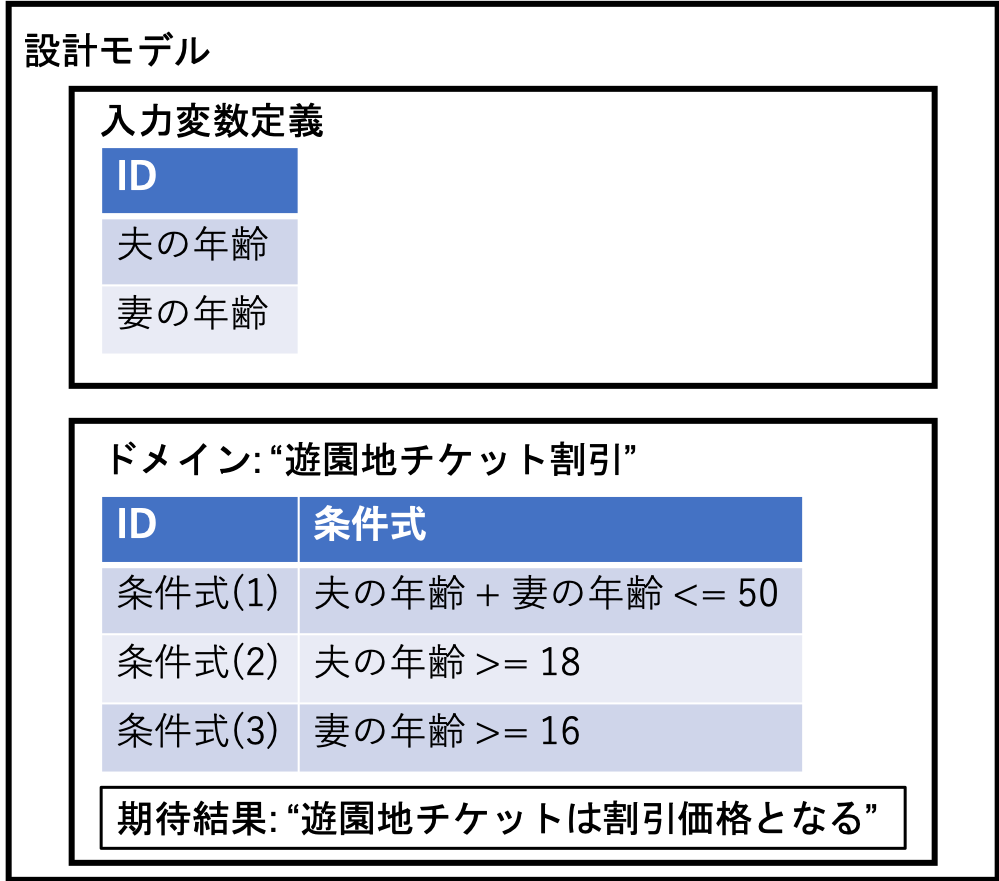
\includegraphics[width=8cm]{image/model_park.png}
    \caption{設計モデルの例(遊園地チケット購入機能)}
    \ecaption{Example of design model (amusement park ticket discount function)}
    \label{fig:model_park}
  \end{center}
\end{figure}
\end{comment}

ドメイン分析に基づいたテストケースを自動生成する手法としては、丹野らの研究\cite{sekkeiModel}がある。
この手法では、変数同士に依存関係がある場合でも、制約ソルバ\cite{sat}を用いることで、依存関係を考慮した境界値等のテストケースを網羅的に生成する。
入力として、ソフトウェアの設計情報をモデル化した設計モデルと呼ばれるテキストを入力する必要がある。
%この設計モデルの例を、\figref{fig:model_park}に示す。これは、\figref{fig:vdm_park}の仕様から設計モデルを作成した例である。
設計モデルは\cite{sekkeiModel}で定義されている。

設計モデルは仕様書を元に、人手で記述する必要があるため、設計モデルの作成に時間と手間がかかってしまうという問題がある。
これに対して、拡張したBWDMは、VDM++仕様を元に、自動でテストケースを生成できるため、設計モデルを作成する必要がないという利点がある。
しかし、仕様書が自然言語のみで記述されている場合、VDM++仕様を記述しなければ、拡張したBWDMを使うことができない。
そのため、自然言語で記述された仕様書からドメイン分析テストのためのテストケースを作成する場合、設計モデルを記述するか、VDM++仕様を記述するかで対応が分かれることとなる。
なお、設計モデルの記述とVDM++仕様の記述に必要な要素がほぼ同じなため、記述量はほとんど変わらないと考える。
設計モデルは丹野らの手法でしか利用できないが、VDM++仕様はBWDM以外にも、VDMTools\cite{vdmtools}やOverture IDE\cite{overture}などの支援ツールが揃っており、仕様の検証や記述を行いやすいという利点がある。

\subsection{複数定義対応に関する評価}
\todo{この節はまだ実験を行っていないため、\ref{sec:domain_exam}節を参考に、文章のみ記述した。
  実験後に、加筆、修正する。}

人手による関数定義、操作定義、定数定義、インスタンス変数定義を含むVDM++仕様のテストケース作成と、拡張したBWDMによるテストケース生成で、作成(生成)に要した時間の比較検証を行った。
その結果を、表\ref{tab:time_definition}に示す。

対象としたVDM++仕様を、コード\ref{fig:multi_definition_exam}に示す。
“割引価格となる”を期待出力に持つドメインに対するドメイン分析テストのためのテストケースを作成する時間を計測した。
生成するテストケースとしては、以下を基準とした。
\begin{enumerate}
  \item 関数X、操作Yのテストケースを出力(記述)する
  \item 境界値の組合せを網羅するテストケースを出力(記述)する。
  \item すべての実行フローを網羅するテストケースを出力(記述)する。
\end{enumerate}

検証に参加したメンバーは本研究室の大学院生X人と学部4年生Y人であり、
普段からソースコードの読み書きを行い、基本的なプログラミングの知識を有している。
VDM++の文法の知識を持たない者も含まれるが、
今回の検証に必要な文法は、事前に他のVDM++の例を用いてレクチャーした。
また、テストケース生成についても、事前に他のVDM++仕様とテストケースの例を用いてレクチャーした。

人手による検証では、コード\ref{fig:multi_definition_exam}を印刷した紙を渡し、
仕様を確認後、テストケースを書き始めてから、テストケースを記述し終えるのに要した時間を計測した。
入力データと期待出力の組み合わせが不正確な場合、間違いを指摘し、
被験者が正しい組み合わせを記述した時点で時間計測終了とした。
また、制限時間を30分とし、制限時間を超えた場合、その場で時間計測終了とした。

拡張したBWDMによる検証では、
コマンドライン上での命令操作で、拡張したBWDMによるテストケース生成を行うのに要した時間を計測した。
また、実験に用いたコンピュータは、OS:macOS 10.15.2、CPU:2.3GHz Intel Core i5、メモリ:16GBである。

なお、JavaのSystem.nanoTime\cite{nanotime}メソッドを用いて、
命令操作を省いた純粋なテストケース生成処理にBWDMが要した時間を計測した結果、
XXXXX秒であった。

人手による作成と比較した結果、平均でYYYY分程の時間短縮を確認できた。
対象にしたVDM++仕様には、VDM++独特の文法等は含まれないため、
VDM++に対する慣れなどの影響は無視できるものと思われる。
また、人手によるテストケース生成の場合、ヒューマンエラーも見られた。
具体的には、〜〜〜〜〜〜を誤って記述してしまった。\todo{ここに例を書く}
仕様の規模が拡大すると、人手とコンピュータとの処理効率の差に加えて、
ヒューマンエラーの有無などにより、テストケース生成に要する時間の差は更に拡大していくと思われる。

\begin{table}[t]
  \begin{center}
    \caption{コード\ref{fig:multi_definition_exam}のテストケース作成に要した時間の比較}
    \label{tab:aaaaaaa}
    \begin{tabular}{c|c}
      被験者 or 拡張したBWDM & 時間  \\
      \hline
      \hline
      被験者A                & 0m 0s \\ \hline
      被験者B                & 0m 0s \\ \hline
      被験者C                & 0m 0s \\ \hline
      被験者D                & 0m 0s \\ \hline
      被験者(平均)           & 0m 0s \\ \hline
      BWDM                   & 0m 0s
    \end{tabular}
  \end{center}
\end{table}



\section{拡張した\tool{}の問題点}
\todo{これからの問題点をかく}

% おわりに
\chapter{おわりに} \label{cha:Conclusion}
\todo{終わりにをかく}

%%
% 謝辞
%
\acknowledgment{}

\todo{謝辞をかく}


%%
% 参考文献
%
\begin{thebibliography}{99}
  % 森氏の成果物
  \bibitem{ICAROB2019} Keisuke Mori, Tetsuro Katayama, Yoshihiro Kita, Hisaaki Yamaba, Kentaro Aburada, and Naonobu Okazaki: ``Development of Library Fescue Extracting Elements of Attributes and Operations of Class Diagram in UML,'' The 2019 International Conference on Artificial Life and Robotics (ICAROB2019), pp. 165--168, 2019

  \bibitem{Fescue} GitHub: ``Fescue: Feature Elements Section of Class in UML Extraction,'' https://github.com/Morichan/Fescue (最終アクセス 2019/01/25)
\end{thebibliography}

%%
% 付録
%
% \appendix{} % 付録は基本的に使わない

\end{document}
